% !TEX program = xelatex
% =============================================================================
%  OceanSwarm GCS 开发文档（中文，XeLaTeX + ctex）
%  编译：xelatex OceanSwarm-GCS-dev-doc.tex（连续两次以生成目录）
% =============================================================================
\documentclass[UTF8, a4paper, 11pt]{ctexart}

\usepackage{geometry}
\geometry{left=2.4cm, right=2.4cm, top=2.6cm, bottom=2.5cm}
\usepackage{graphicx}
\usepackage{xcolor}
\usepackage{colortbl}
\usepackage{amsmath}
\usepackage{amssymb}
\usepackage{booktabs}
\usepackage{array}
\usepackage{multirow}
\usepackage{caption}
\usepackage{subcaption}
\usepackage{float}
\usepackage{longtable}
\usepackage{fancyhdr}
\usepackage{tikz}
\usetikzlibrary{arrows.meta, positioning, shapes.geometric, calc}
\usepackage{listings}
\usepackage{hyperref}

\definecolor{themeblue}{HTML}{1C5A96}
\definecolor{themecoral}{HTML}{E08F96}
\definecolor{themecyan}{HTML}{2BC8C0}
\definecolor{themegray}{HTML}{4A5A66}
\definecolor{themegold}{HTML}{C9973F}
\definecolor{codebg}{HTML}{F4F7FA}
\definecolor{codeframe}{HTML}{C8D6E2}
\definecolor{linkcolor}{HTML}{1565A8}

\hypersetup{
  colorlinks=true,
  linkcolor=themeblue,
  citecolor=themeblue,
  urlcolor=linkcolor,
  pdftitle={OceanSwarm GCS 无人艇集群地面指挥控制上位机开发文档},
  pdfauthor={朱华天},
  pdfsubject={无人艇集群上位机、Three.js 三维海域视景与 3-DOF 水动力动力学},
  pdfkeywords={USV, GCS, 无人艇集群, Three.js, Vite, 3-DOF 水动力学, 动力定位, 实时渲染}
}

\captionsetup{font=small, labelsep=quad}
\captionsetup[subfigure]{font=small}

\pagestyle{fancy}
\fancyhf{}
\fancyhead[L]{\small\color{themegray}OceanSwarm GCS 开发文档}
\fancyhead[R]{\small\color{themegray}\thepage}
\setlength{\headheight}{22pt}
\renewcommand{\headrulewidth}{0.3pt}
\renewcommand{\headrule}{\hbox to\headwidth{\color{codeframe}\leaders\hrule height \headrulewidth\hfill}}

\lstdefinestyle{code}{
  backgroundcolor=\color{codebg},
  frame=single,
  rulecolor=\color{codeframe},
  basicstyle=\ttfamily\footnotesize,
  keywordstyle=\color{themeblue}\bfseries,
  commentstyle=\color{themegray}\itshape,
  stringstyle=\color{themecoral!80!black},
  numbers=left,
  numberstyle=\tiny\color{themegray},
  numbersep=7pt,
  breaklines=true,
  columns=fullflexible,
  keepspaces=true,
  showstringspaces=false,
  tabsize=2,
  aboveskip=8pt,
  belowskip=8pt,
  xleftmargin=1.4em,
  framexleftmargin=1.2em
}
\lstset{style=code}

\newcommand{\file}[1]{\texttt{#1}}
\newcommand{\repolink}{\href{https://github.com/ZHT1235456/OceanSwarm-GCS}{\texttt{https://github.com/ZHT1235456/OceanSwarm-GCS}}}
\emergencystretch=1.2em

% =============================================================================
\begin{document}
\sloppy

% ============================= 封面 =========================================
\begin{titlepage}
\centering
\vspace*{0.9cm}
{\color{themeblue}\rule{\linewidth}{1.2pt}}\\[0.8cm]
{\huge\bfseries\color{themeblue} 无人艇集群地面指挥控制上位机}\\[0.5cm]
{\LARGE OceanSwarm GCS 开发文档}\\[0.5cm]
{\large Three.js 海域视景 · 仿真数据链 · 3-DOF 水动力动力学}\\[0.6cm]
{\color{themeblue}\rule{\linewidth}{1.2pt}}\\[1.0cm]

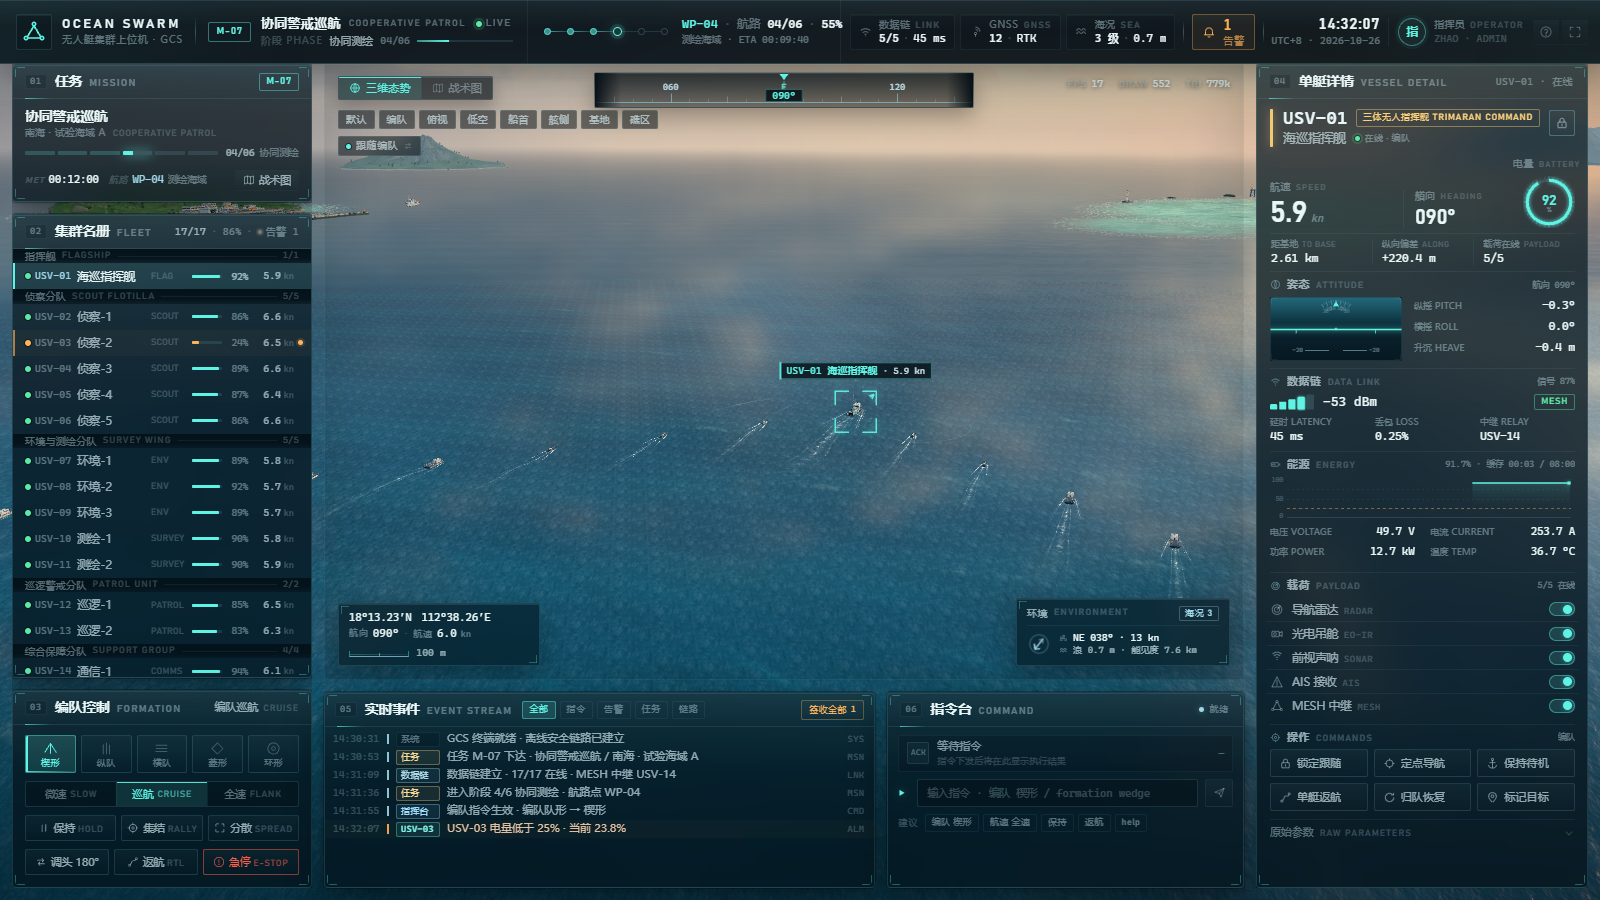
\includegraphics[width=0.94\linewidth]{figures/gcs-01-console.png}\\[0.9cm]

{\large
\begin{tabular}{rl}
\textbf{项目：} & OceanSwarm GCS（v2.1） \\[0.3em]
\textbf{作者：} & 朱华天 \\[0.3em]
\textbf{模型：} & DeepSeek V4.1 Flash 1017 \\[0.3em]
\textbf{日期：} & 2026 年 10 月 26 日 \\[0.3em]
\textbf{仓库：} & \repolink \\
\end{tabular}}
\vfill
{\small\color{themegray}17 艘无人水面艇 \quad|\quad Three.js 0.186 \quad|\quad Vite 7 \quad|\quad 完全离线运行}
\end{titlepage}

% ============================= 摘要 =========================================
\pagenumbering{Roman}
\begin{abstract}
\noindent
本文件记录 OceanSwarm GCS v2.1 的设计与实现。项目面向 17 艘无人水面艇组成的集群，交付一套可在浏览器中直接运行的地面指挥控制上位机。界面包含顶栏、集群名册与任务卡、编队控制、三维态势视景、二维战术图、单艇详情、实时事件流与指令台、开机自检与急停覆盖层，共七个区域。仿真层以 10~Hz 生成遥测、数据链、告警与指令回执；操作员下达的编队、航速、保持、调头、返航、急停与单艇派遣指令经模拟链路延时后进入场景执行，执行结果写回事件流与面板。三维视景继承 OceanSwarm 海域场景，包含程序化海面、HDR 天空、17 艘参数化无人艇、尾迹与环境设施。v2.1 将每艘艇的运动替换为纵荡、横荡、艏摇三个自由度的水动力操纵模型，模型包含刚体质量与附加质量、线性与二次阻尼、推力滞后、舵机限幅、水流相对速度以及低速动力定位执行器。编队保持、航点到达、返航与急停由制导、自动舵和积分器闭环完成，界面显示的航速、舵角、油门、漂角与航迹向均为模型输出。文档依次介绍运行方式、系统架构、继承的三维视景、上位机界面、仿真数据链、编队控制、水动力模型、性能与质量验证，并附参数表、目录结构与素材许可。全部内容离线运行；生产构建约 5.69~MB；整机回归 30 项断言通过，水动力自测 141 项、闭环与编队集成测试全部通过。

\vspace{0.6em}
\noindent\textbf{关键词：} 无人水面艇；地面指挥控制站；集群控制；Three.js；Vite；3-DOF 水动力模型；动力定位
\end{abstract}

\newpage
\tableofcontents
\newpage

% ============================= 正文 =========================================
\pagenumbering{arabic}
\setcounter{page}{1}

% -----------------------------------------------------------------------------
\section{项目概述}

\subsection{项目背景}

OceanSwarm 最初是一个三维海域场景项目：半径约 26~km 的开放海面、一支按任务类型编组的无人艇集群、由本地 HDR 全景驱动的天空与海面，以及海岛、试验基地、珊瑚礁等环境。场景本身可以自由观察，缺少指挥操作所需的信息组织、指令通道与数据反馈。

本项目在该场景上构建地面指挥控制上位机（Ground Control Station，GCS）。系统面向 17 艘无人水面艇，操作员在浏览器中完成三类工作：查看集群与单艇状态，向集群或单艇下达任务指令，确认指令执行结果与告警。三维场景承担态势呈现和运动执行，仿真层承担遥测生成、链路模拟与告警判定，界面层只负责显示与交互。

v2.1 的重点是运动真实性。此前的编队采用质点式跟随，位置直接趋近目标点，航速等于指令值。当前版本为每艘艇建立水动力操纵模型，控制器输出油门、舵角与侧推指令，位置、艏向与速度由模型积分得到。编队变化、单艇派遣、返航和急停因此具有加速过程、惯性、转弯半径与滑行距离。

\subsection{交付内容}

\begin{itemize}
  \item \textbf{三维海域视景}：程序化海面、HDR 天空与光照、17 艘参数化无人艇、尾迹与泡沫、海岛与试验基地、珊瑚礁潟湖、航标与风机等环境要素。
  \item \textbf{七个界面区域}：顶栏、左栏（任务与名册、编队控制）、中央三维态势与二维战术图、右栏（单艇详情）、底栏（事件流与指令台）、覆盖层（开机、急停、帮助、Toast）。
  \item \textbf{仿真与数据链}：10~Hz 遥测快照、分组与航路、链路延时与丢包、电量与温度演化、五类告警规则、事件环形缓冲、指令校验与回执。
  \item \textbf{编队与单艇控制}：五种队形、三档航速、编队保持与恢复、集结与分散、调头、返航、集群急停、单艇派遣与待机。
  \item \textbf{3-DOF 水动力动力学}：8 型艇的质量、附加质量、阻尼、推力、舵机、水流与低速动力定位模型，以及配套的制导与自动舵。
  \item \textbf{验证资产}：整机截图回归、仿真与水动力自测、编队集成测试脚本，以及文档插图使用的截图基线。
\end{itemize}

\begin{figure}[H]
  \centering
  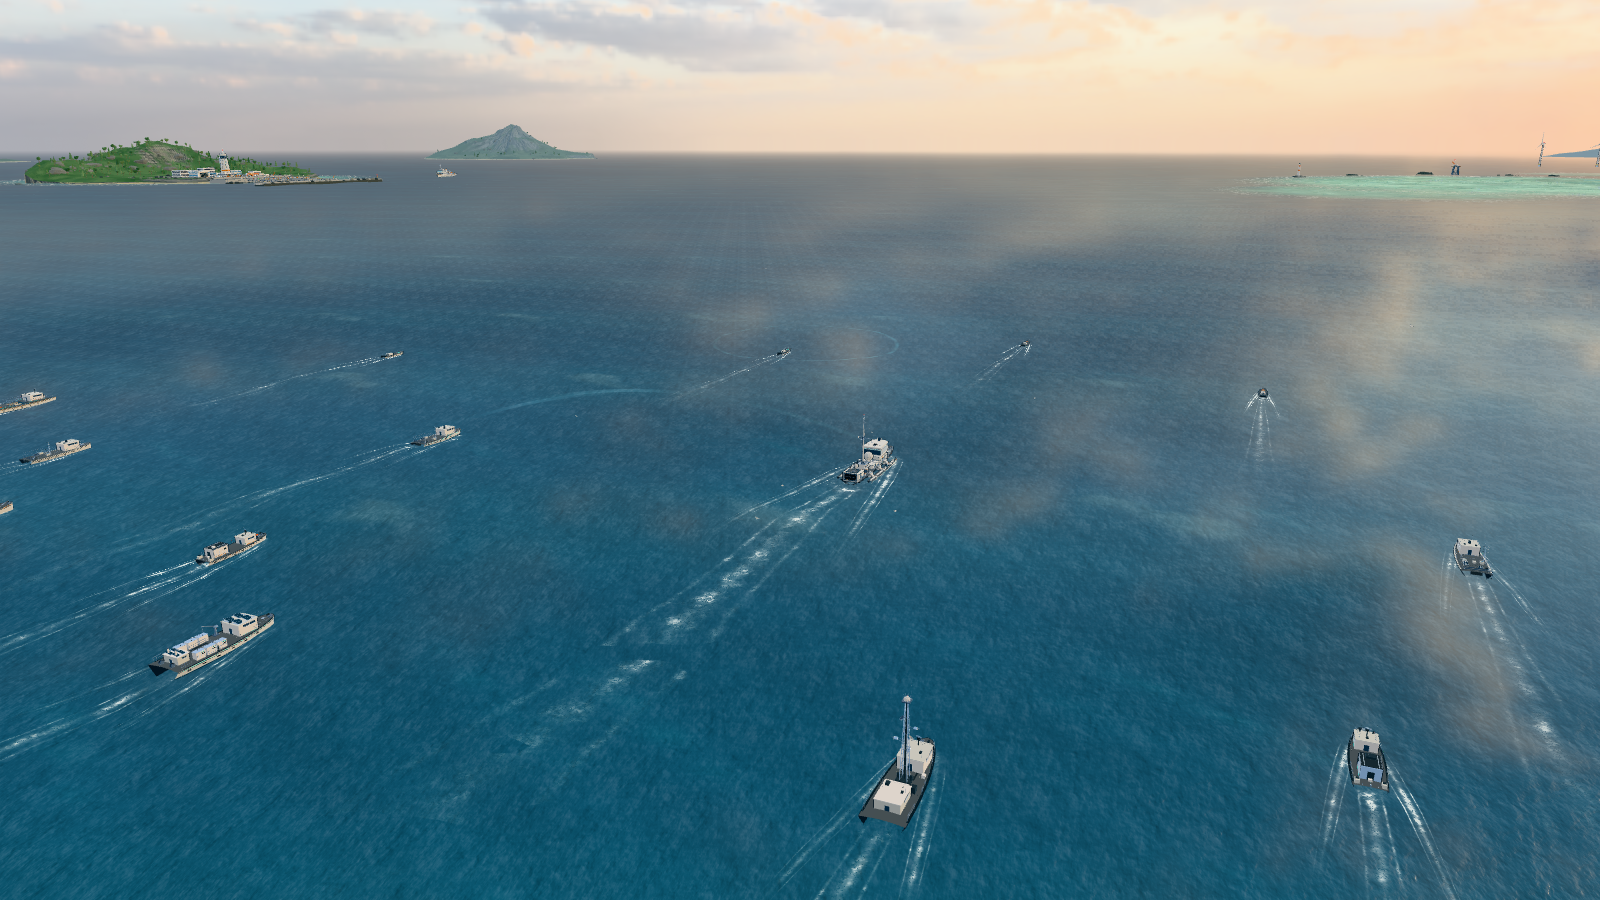
\includegraphics[width=\linewidth]{figures/fig-00-hero.png}
  \caption{继承的 OceanSwarm 三维海域视景。}
  \label{fig:hero}
\end{figure}

\subsection{需求与实现}

\begin{table}[H]
\centering
\caption{需求与实现方式}
\label{tab:req-map}
\small
\begin{tabular}{@{}p{0.28\linewidth}p{0.64\linewidth}@{}}
\toprule
\textbf{需求} & \textbf{实现} \\
\midrule
集群上位机界面 & \file{src/ui/} 七个面板与 shell/context 骨架，面板动态加载 \\
指令闭环 & \file{src/sim/commands.js} 校验、延时、回执；\file{src/systems/swarm-control.js} 执行 \\
17 艇遥测 & 10~Hz 快照；名册、三维锁定框、战术图与右栏同步选中 \\
二维战术图 & Canvas2D 海图：经纬网、距离环、岛礁与基地、航路、17 艇标、航点工具 \\
真实运动 & \file{vessel-dynamics.js} 三自由度水动力模型与积分器 \\
编队与航速 & 阵位生成、制导、自动舵、动力定位闭环 \\
急停与告警 & 推进切断与滑行；五类告警带持续判据与恢复事件 \\
离线运行 & 本地 HDR 与水面法线贴图；无外部字体、图标库或 CDN \\
\bottomrule
\end{tabular}
\end{table}

% -----------------------------------------------------------------------------
\section{运行与操作}

\subsection{环境与命令}

运行环境为 Node.js 18 及以上版本，依赖 \file{three@0.186} 与 \file{vite@7}。两张本地素材随仓库提供：天空 HDR 全景 4\,434\,394 字节，水面法线贴图 248\,813 字节。素材通过应用自身的 base URL 加载，运行时不访问外部网络。HDR 缺失时回退到程序化天空，水面法线缺失时回退到程序化涟漪。

\begin{lstlisting}[language=bash, caption={安装、运行与质量验证命令}, label={lst:run}]
npm install
npm run dev      # 开发服务器 http://127.0.0.1:5179
npm run build    # 生产构建，输出到 dist/
npm run preview  # 预览生产构建 http://127.0.0.1:5180

npm run qa:gcs       # 整机截图与交互回归（30 断言）
npm run qa:dynamics  # 水动力模型自测（141 项）
npm run qa:motion    # plant 与 autopilot 闭环自测（10 项）
npm run qa:fleet     # 真实 Fleet 与 SwarmControl 集成自测（13 项）
npm run qa:sim       # 仿真、数据链、告警与指令总线自测（32 项）
\end{lstlisting}

生产构建目标为 es2022，主程序使用顶层 await 预加载 HDR 与水面法线贴图。v2.1 的 \file{dist/} 合计约 5.69~MB，其中主 JavaScript 约 707~KB（gzip 约 207~KB），按面板拆分的懒加载块若干，HDR 资源 4.43~MB，水面法线 249~KB。

\subsection{控制台操作}

\begin{itemize}
  \item 选中：点击三维海面上的艇、左栏名册行或战术图艇标。双击名册行或三维艇进入锁定跟随。
  \item 视角：左键拖拽旋转，滚轮缩放，右键拖拽平移。右上角 HUD 提供八种视角预设，\texttt{F} 锁定或解除锁定，\texttt{R} 返回编队跟随。
  \item 编队：\texttt{1}--\texttt{5} 切换队形，\texttt{Shift+1/2/3} 选择微速、巡航、全速，\texttt{Space} 保持或恢复，\texttt{U} 调头。
  \item 视图：\texttt{M} 在三维态势与二维战术图之间切换，\texttt{H} 隐藏面板进入纯净视景，\texttt{?} 打开帮助。
  \item 指令台：输入中英文命令并回车。支持 \texttt{Tab} 补全、上下键历史与建议按钮。命令示例：\texttt{编队 纵队}、\texttt{formation column}、\texttt{航速 全速}、\texttt{返航}、\texttt{goto 900 -200}、\texttt{select scout-2}。
\end{itemize}

\begin{table}[H]
\centering
\caption{调试与截图用 URL 参数}
\label{tab:urlparams}
\small
\begin{tabular}{@{}l p{0.64\linewidth}@{}}
\toprule
\textbf{参数} & \textbf{作用} \\
\midrule
\file{?nointro=1} & 跳过开机自检动画 \\
\file{?seed=7} & 固定仿真随机种子，保证遥测与截图可复现 \\
\file{?view=<name>} & 初始相机预设（default、fleet、top、low、bow、side、base、reef） \\
\file{?bootms=6000} & 放慢开机动画，用于截取开机状态 \\
\bottomrule
\end{tabular}
\end{table}

\subsection{视角与镜头}

默认镜头位于编队质心后方约 600~m、上方约 190~m、右方约 190~m，视场角 47$^\circ$，俯角约 16$^\circ$。镜头有三种导演模式：跟随编队、锁定选中艇、自由观察。跟随编队模式随质心平移，保持构图稳定；锁定模式平滑转向目标并跟随其运动。八种预设覆盖全景、低角度、船首、舷侧、编队俯视、基地与珊瑚礁等取景需求。

\begin{figure}[H]
  \centering
  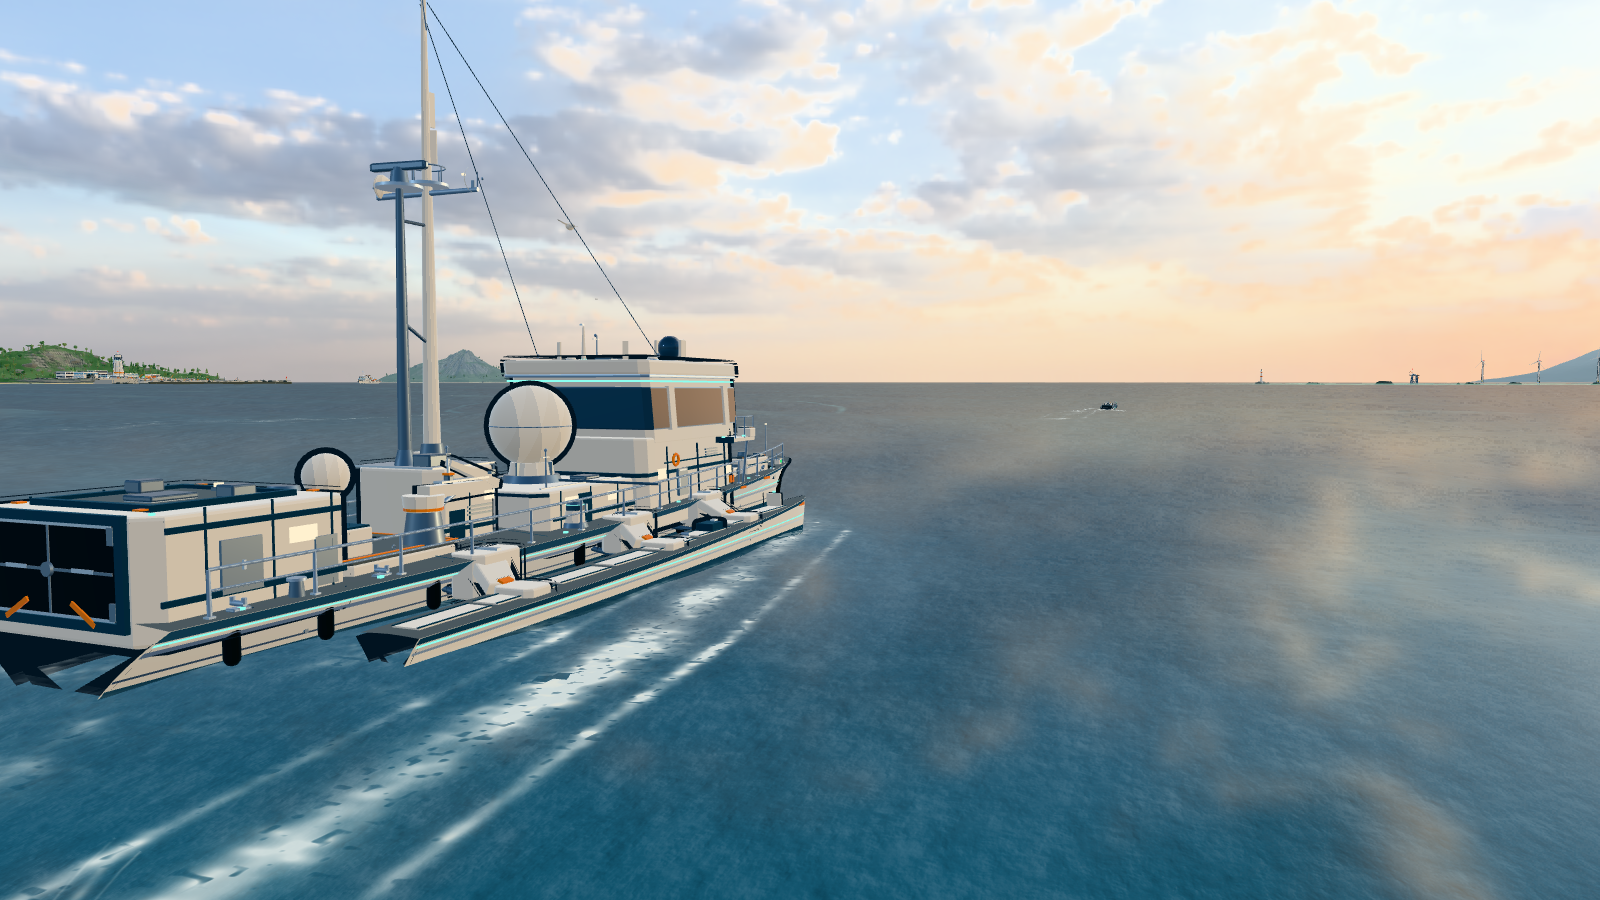
\includegraphics[width=0.95\linewidth]{figures/fig-01-low-angle.png}
  \caption{水面低角度视角：旗舰舷侧、泡沫水线与落日海面。}
  \label{fig:low}
\end{figure}

% -----------------------------------------------------------------------------
\section{系统架构}

\subsection{分层结构}

代码按四层组织：界面层、仿真数据层、指挥控制层与视景层。图层之间只有一个方向的数据流动，界面层读取仿真快照并派发语义动作，不直接修改场景对象。

\begin{itemize}
  \item \textbf{界面层} \file{src/ui/}：\file{shell.js} 建立区域骨架，\file{context.js} 提供 UI 状态、动作分发、事件总线与弹层服务，\file{panels/} 包含七个面板，\file{charts.js} 提供 Canvas 仪表，\file{styles/} 存放设计变量与面板样式。
  \item \textbf{仿真数据层} \file{src/sim/}：\file{model.js} 维护 17 艇遥测与任务阶段，\file{commands.js} 处理指令校验与链路，\file{alarms.js} 维护告警生命周期，\file{events.js} 维护事件缓冲，其余模块提供时钟、随机数、领域常量与格式化。
  \item \textbf{指挥控制层} \file{src/systems/} 与 \file{src/gcs/}：\file{swarm-control.js} 负责阵位与任务状态，\file{vessel-dynamics.js} 提供水动力 plant，\file{motion-controller.js} 提供制导与自动舵，\file{camera-director.js} 负责镜头，\file{scene-bridge.js} 提供场景真值适配，\file{meta.js} 存放任务、名册、队形与载荷常量。
  \item \textbf{视景层}：\file{main.js} 完成渲染器、相机、灯光与场景装配；\file{core/} 提供几何、HDR、材质、波场、海面与天空；\file{objects/} 提供船体、环境与特效；\file{systems/formation.js} 提供航线与随浪姿态。
\end{itemize}

\begin{figure}[H]
\centering
\begin{tikzpicture}[
  font=\footnotesize,
  layer/.style={draw=themeblue!55, fill=themeblue!7, rounded corners=2pt, align=left, inner sep=4pt, text width=12.4cm},
  arr/.style={-{Stealth[length=2.2mm]}, draw=themegray, line width=0.6pt}
]
\node[layer, fill=themecoral!10, draw=themecoral!70] (ui) at (0,5.6) {\textbf{界面层} \file{src/ui/}：shell、context、七个面板、Canvas 仪表与样式};
\node[layer, fill=themecyan!10, draw=themecyan!70] (sim) at (0,4.1) {\textbf{仿真数据层} \file{src/sim/}：遥测模型、指令总线、告警、事件、时钟};
\node[layer, fill=themegold!14, draw=themegold!70] (ctl) at (0,2.6) {\textbf{指挥控制层} \file{src/systems} 与 \file{src/gcs}：编队控制、水动力 plant、制导与自动舵、镜头、场景桥};
\node[layer, fill=themegray!10, draw=themegray!70] (scene) at (0,1.1) {\textbf{视景层（继承）}：\file{main.js}、\file{core/}、\file{objects/}、航线与随浪姿态};
\draw[arr, -{Stealth[length=2.2mm]}, draw=themegray, line width=0.6pt] (scene.north) -- (ctl.south);
\draw[arr, -{Stealth[length=2.2mm]}, draw=themegray, line width=0.6pt] (ctl.north) -- (sim.south);
\draw[arr, -{Stealth[length=2.2mm]}, draw=themegray, line width=0.6pt] (sim.north) -- (ui.south);
\end{tikzpicture}
\caption{四层架构。场景真值向上汇聚为快照，用户指令向下进入控制层。}
\label{fig:arch}
\end{figure}

\subsection{帧循环}

渲染循环每帧按固定顺序执行：

\begin{enumerate}
  \item 计算帧间隔 \texttt{dt}，上限 0.1~s；暂停状态下 \texttt{dt} 取 0，相机与界面仍可操作。
  \item \file{fleet.update(dt)} 推进航路，计算阵位目标，运行制导与自动舵，积分水动力状态，更新船体矩阵与随浪姿态。
  \item \file{swarm.update(dt)} 处理队形补间、航速与保持状态、单艇到达判据与机动标志。
  \item 更新相机导演与选中光效，调用 \file{scene.updateMatrixWorld()}。
  \item 更新尾迹与泡沫、通信光效、海鸥，以及海岛、珊瑚礁、基地、母船与航标动画。
  \item 更新海面与天空（跟随相机），执行 \file{renderer.render()}。
  \item \file{sim.update} 生成快照，七个面板读取快照并更新 DOM 与 Canvas；调试钩子 \file{window.\_\_gcs} 对外暴露状态与截图方法。
\end{enumerate}

\begin{figure}[H]
\centering
\begin{tikzpicture}[
  font=\small,
  flowstep/.style={draw=themeblue!55, fill=themeblue!6, rounded corners=2pt, align=left, inner sep=4pt, text width=12.4cm},
  arr/.style={-{Stealth[length=2.2mm]}, draw=themegray, line width=0.6pt}
]
\node[flowstep] (s1) {1. 帧间隔与模拟时钟};
\node[flowstep, below=0.1cm of s1] (s2) {2. 舰队水动力、制导与自动舵积分};
\node[flowstep, below=0.1cm of s2] (s3) {3. 编队指挥状态与单艇任务};
\node[flowstep, below=0.1cm of s3] (s4) {4. 镜头、选中光效与世界矩阵};
\node[flowstep, below=0.1cm of s4] (s5) {5. 尾迹、光效与场景环境动画};
\node[flowstep, below=0.1cm of s5] (s6) {6. 海面、天空与最终渲染};
\node[flowstep, below=0.1cm of s6] (s7) {7. 仿真快照与七个面板更新};
\foreach \a/\b in {s1/s2, s2/s3, s3/s4, s4/s5, s5/s6, s6/s7} \draw[arr] (\a) -- (\b);
\end{tikzpicture}
\caption{每帧执行顺序。}
\label{fig:loop}
\end{figure}

\subsection{数据契约}

仿真快照是界面层唯一的数据来源，包含以下分组：

\begin{table}[H]
\centering
\caption{快照分组与关键字段}
\label{tab:snapshot}
\small
\begin{tabular}{@{}p{0.16\linewidth}p{0.76\linewidth}@{}}
\toprule
\textbf{分组} & \textbf{字段} \\
\midrule
fleet & centerX、centerZ、headingDeg、speedKn（17 艇对地速度均值）、mode、formationKey、estopActive、formationTransition、manoeuvring \\
vessels[] & id、type、group、x、z、headingDeg、sogKn、uKn、swayKn、cogDeg、driftDeg、yawRateDegS、rudderDeg、throttlePct、batteryPct、link、sensors、stationErrorM、mode \\
mission & phaseIndex、waypointIndex、MET 文本与航路点名称 \\
events、alarms、acks & 事件流、活动告警与签收状态 \\
system & 帧率、绘制调用、三角形数量、模拟时间 \\
\bottomrule
\end{tabular}
\end{table}

指令对象包含 \texttt{type} 与参数，例如 \texttt{\{type:'formation.set', formation:'column'\}} 或 \texttt{\{type:'vessel.goto', id:'scout-2', x, z\}}。界面层通过 \file{context.actions} 或指令台产生指令，仿真层完成校验、延时与回执。

\subsection{代码规模}

v2.1 仓库含 62 个 JavaScript 与 CSS 源文件，约 37\,600 行（不含依赖）。

\begin{table}[H]
\centering
\caption{主要源文件}
\label{tab:files}
\footnotesize
\begin{tabular}{@{}p{0.34\linewidth}r p{0.44\linewidth}@{}}
\toprule
\textbf{文件} & \textbf{行数} & \textbf{职责} \\
\midrule
\file{src/ui/}（index、context、shell） & 1\,050 & UI 根、状态与动作总线、区域骨架、键盘、调试钩子 \\
\file{src/ui/panels/}（7 个） & 6\,800 & 顶栏、左栏、HUD、战术图、右栏、底栏、覆盖层 \\
\file{src/ui/charts.js} 与 \file{src/ui/styles/} & 8\,500 & Canvas 仪表；设计变量、基础组件与面板样式 \\
\file{src/sim/}（8 个） & 3\,600 & 遥测模型、数据链、告警、事件、时钟与随机数 \\
\file{src/systems/vessel-dynamics.js} & 739 & 三自由度水动力 plant \\
\file{src/systems/motion-controller.js} & 320 & 制导、速度环、艏向环、航点包线与动力定位 \\
\file{src/systems/swarm-control.js} & 560 & 阵位、航速、保持、调头、返航、急停与单艇任务 \\
\file{src/gcs/meta.js} 与 \file{src/gcs/scene-bridge.js} & 570 & 任务、名册、队形、载荷常量与场景真值适配 \\
\file{src/systems/camera-director.js} 与选中光效 & 260 & 镜头导演、选中框、航点光柱与派遣航线 \\
\file{src/main.js} & 560 & 场景装配、GCS 集成、镜头、拾取与暂停钩子 \\
\file{src/config.js} & 277 & 调色板、世界布局、编队名册、相机与水流参数 \\
\file{src/core/}（8 个） & 2\,000 & 几何、HDR、材质、波场、海面、天空、水法线 \\
\file{src/systems/formation.js} & 320 & 航线、阵位与随浪姿态 \\
\file{src/objects/}（船体、环境、特效） & 13\,500 & 17 艘船、海岛、珊瑚礁、基地、母船、航标、尾迹与光效 \\
\bottomrule
\end{tabular}
\end{table}

\subsection{坐标与单位}

场景采用米制单位，$+X$ 向东、$+Y$ 向上、$+Z$ 向南。船体局部坐标中 $+X$ 为船首、$+Z$ 为右舷。艏向角 $\psi=0$ 时船首指向 $+X$，正 $\psi$ 为左转，运动学关系为
\begin{equation}
\dot x=\cos\psi\,u+\sin\psi\,v,\qquad
\dot z=-\sin\psi\,u+\cos\psi\,v,\qquad
\dot\psi=r .
\end{equation}
界面显示罗经航向，与 $\psi$ 的换算关系为$90^\circ-\psi$。

% -----------------------------------------------------------------------------
\section{三维海域视景}

\subsection{海面}

海面由七组方向波叠加而成，采样函数为
\begin{equation}
y(\mathbf p,t)=\sum_{i=1}^{7}A_i\sin\!\left(k_i\,\mathbf d_i\cdot\mathbf p-\omega_i t+\varphi_i\right),
\qquad k_i=\frac{2\pi}{\lambda_i},
\label{eq:waves}
\end{equation}
其中 $\mathbf p=(x,z)$ 为水平位置，$\lambda_i$ 覆盖 132~m 到 5.6~m 的波段。CPU 采样用于船体随浪姿态，GLSL 端使用同一组参数计算几何起伏，两者保持一致。

海面网格采用径向加密的环形网格，随相机移动，远处网格间距增大。着色器叠加三层拉伸漂移的照片法线细节，模拟近景毛细波、中景细浪与远景风斑；水体颜色以暗色基底加环境反射为主，菲涅尔项控制反射强度，距离雾按视线方向采样 HDR 地平线颜色，使海天交界线保持连续。

\subsection{天空与光照}

天空穹顶使用等距圆柱映射采样本地 2K HDR 全景。全景同时提供三份数据：穹顶像素、海面反射方向采样、PMREM 环境图。太阳方位角与仰角从全景图像中测得，与平行光方向对齐。雾色取地平线方向的全景平均色。场景关闭实时阴影，船体体积由尾迹泡沫、水线压暗和边缘光表达。

\begin{figure}[H]
  \centering
  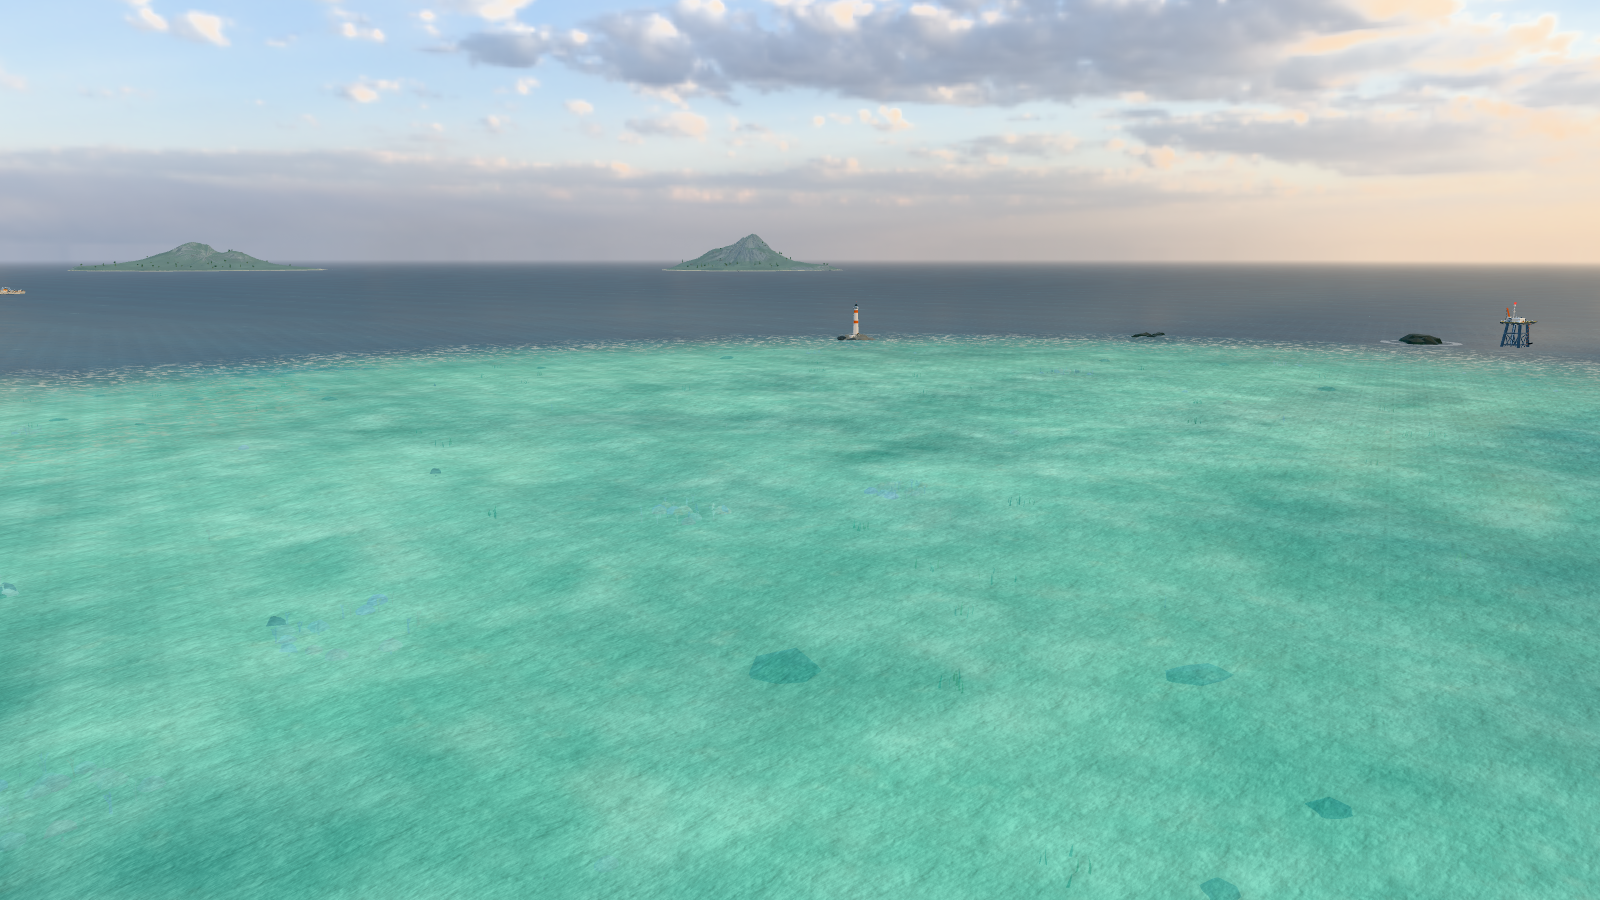
\includegraphics[width=0.95\linewidth]{figures/fig-04-reef.png}
  \caption{珊瑚礁潟湖浅水区。}
  \label{fig:reef}
\end{figure}

\subsection{无人艇建模}

17 艘艇由参数化几何生成，分为旗舰、侦察、环境、测绘、巡逻、通信、能源、救援八类。船体、上层建筑、设备与舷侧细节按材质键合批，单艇约 20--25 次绘制调用；需要动画的雷达、光电云台和航行灯单独成组。旗舰为 30~m 三体结构，13 个材质批次与描边，约 6.1 万三角形。

\begin{figure}[H]
  \centering
  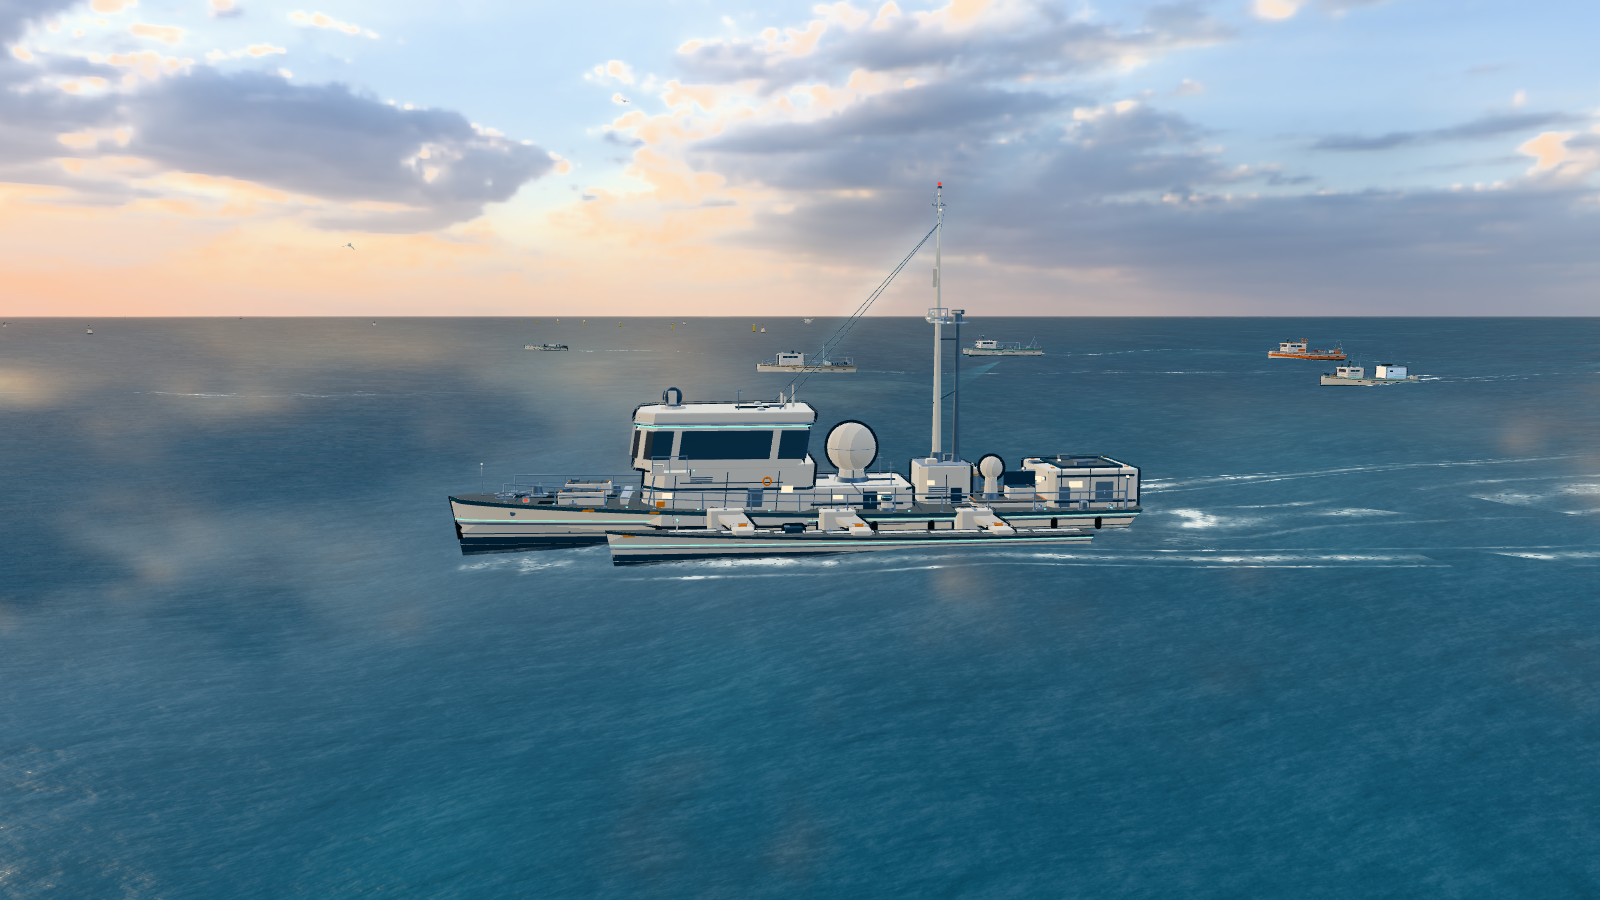
\includegraphics[width=0.95\linewidth]{figures/fig-07-side.png}
  \caption{旗舰右舷近景。}
  \label{fig:side}
\end{figure}

\subsection{尾迹与环境}

每艘艇维护一条历史轨迹带与破浪泡沫网格。轨迹带按航迹保留最近一段时间的点，顶点宽度随船速变化；船首 V 形泡沫由距离船首的距离与横向偏移计算透明度，尾流泡沫使用噪声与时间衰减。环境部分包含左侧试验基地与 120~m 保障母船、右前方珊瑚礁潟湖、三座海岛、航标浮标阵列、灯塔、自升式观测平台与五台海上风机。

\begin{figure}[H]
  \centering
  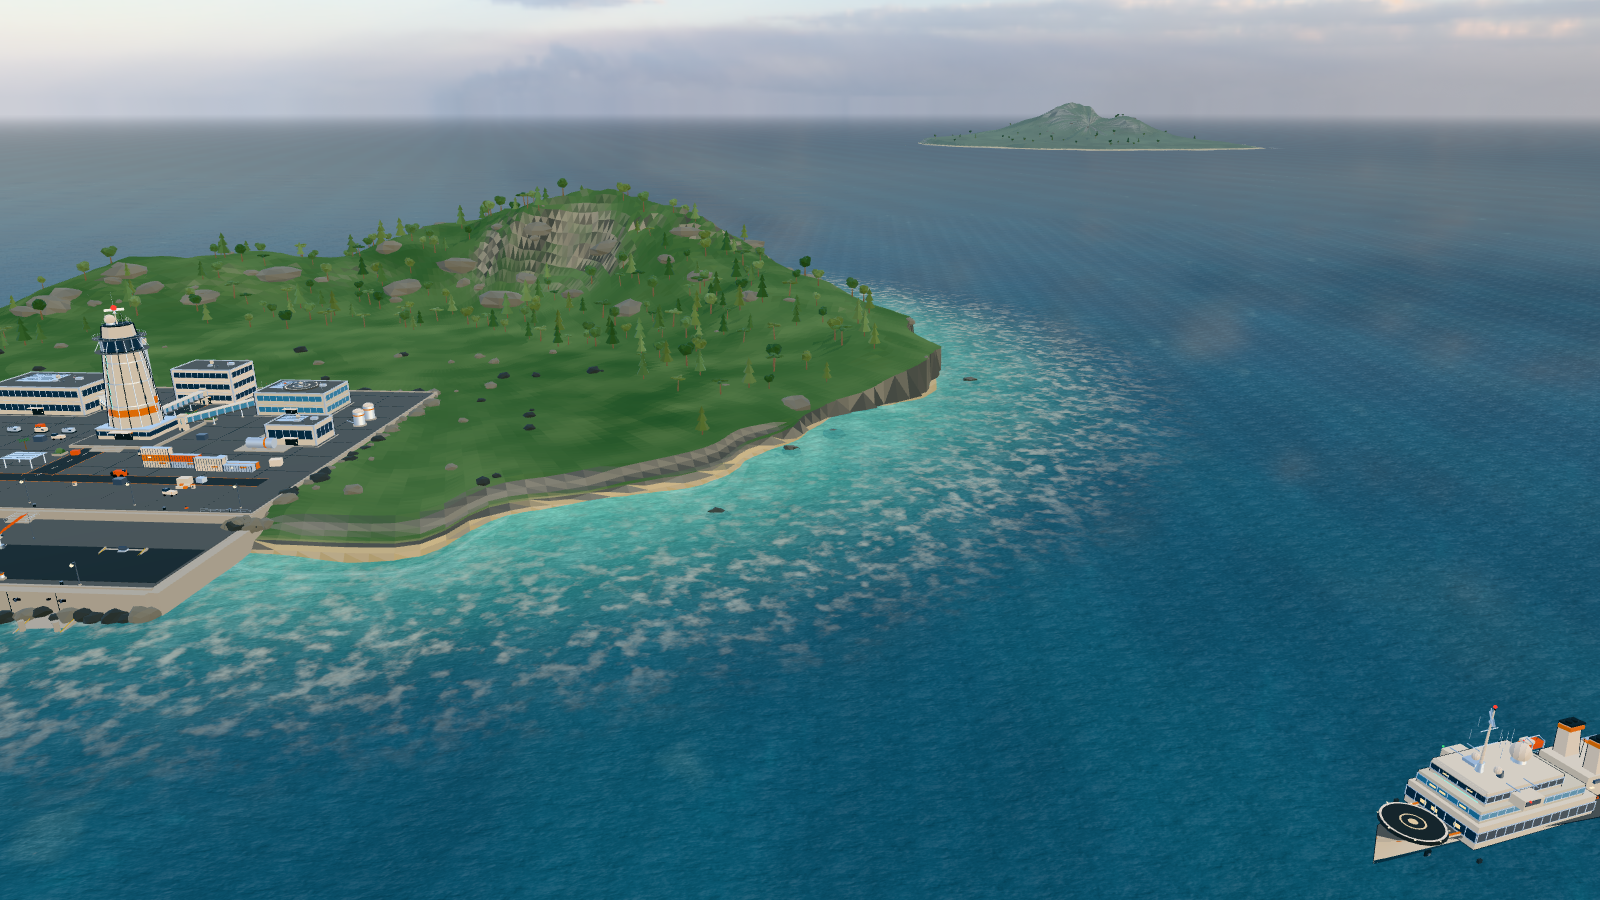
\includegraphics[width=0.95\linewidth]{figures/fig-03-base.png}
  \caption{试验基地与保障母船。}
  \label{fig:base}
\end{figure}

% -----------------------------------------------------------------------------
\section{上位机界面}

\subsection{设计目标}

界面需要在海面视景之上保持可读性，同时承载 17 艘艇的密集信息。设计采用深色玻璃面板、细发丝线、等宽数字与中英双语微标签。颜色语义固定：青蓝色用于选中与导航，琥珀色用于注意与告警，珊瑚红用于急停与严重告警，灰蓝色用于辅助说明。设计变量、组件与状态样式记录在 \file{docs/GCS-design-system.md}。

界面字体使用系统字体栈，图标以内联 SVG 绘制。所有资源随应用打包，页面在离线环境下可完整显示。

\subsection{区域布局}

\begin{figure}[H]
  \centering
  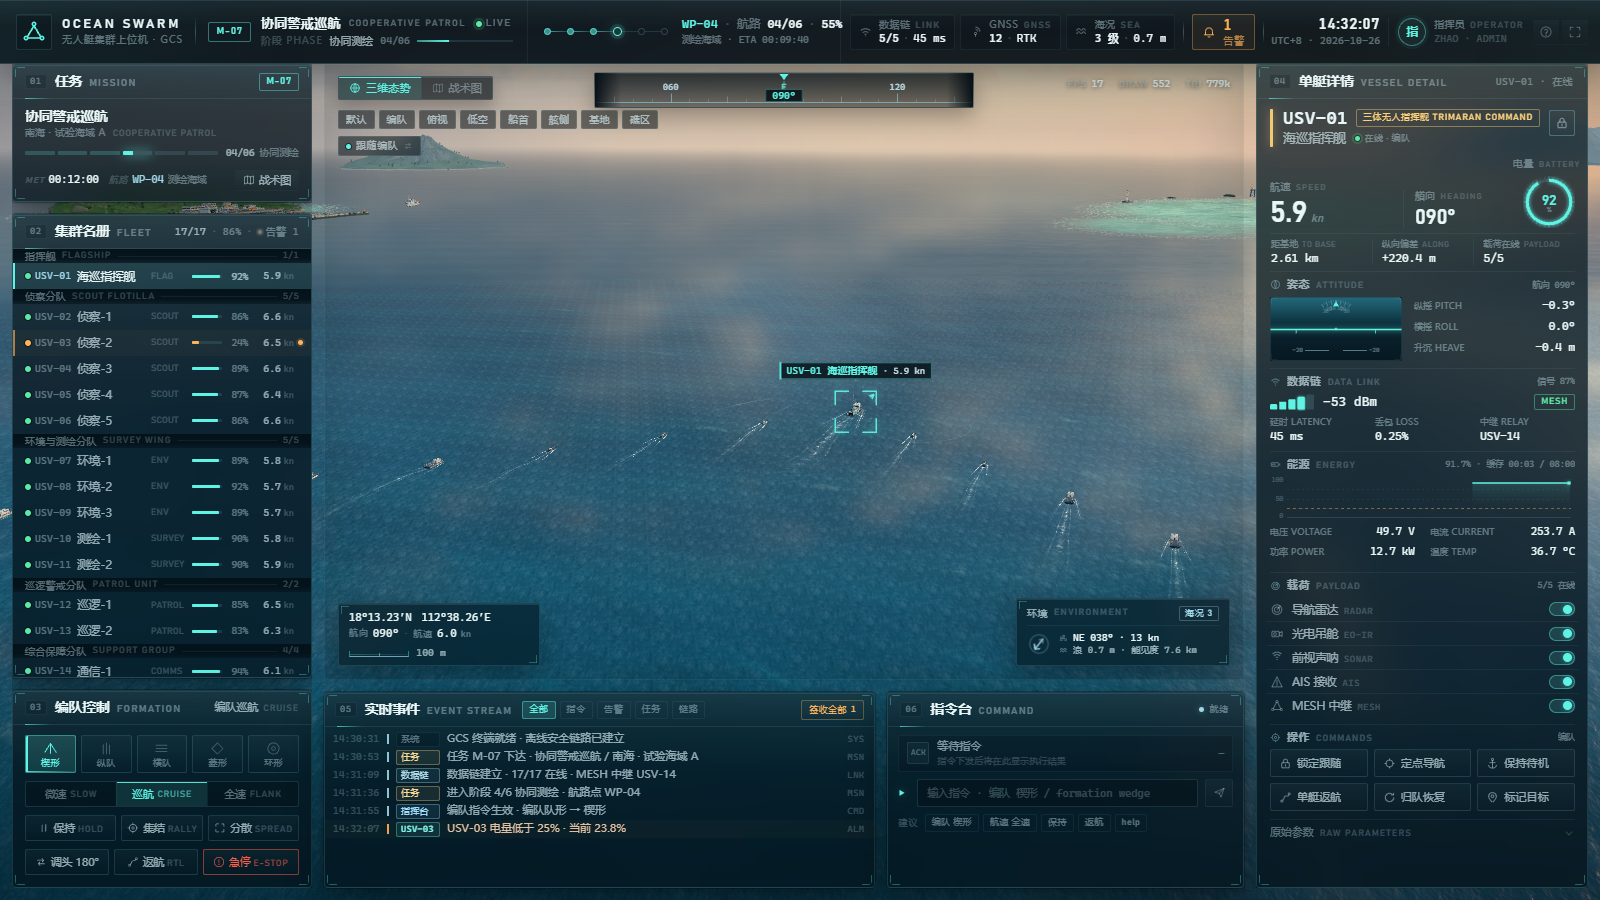
\includegraphics[width=\linewidth]{figures/gcs-01-console.png}
  \caption{默认视图。中央为三维态势，四周为任务、名册、编队、详情、事件与指令台面板。}
  \label{fig:console}
\end{figure}

\begin{table}[H]
\centering
\caption{七个区域的职责}
\label{tab:gcs-layout}
\small
\begin{tabular}{@{}p{0.15\linewidth}p{0.50\linewidth}p{0.27\linewidth}@{}}
\toprule
\textbf{区域} & \textbf{内容} & \textbf{操作} \\
\midrule
顶栏 & 徽标、任务 M-07、阶段与航路进度、数据链状态、GNSS、海况、告警计数、UTC+8 时钟、指挥员、帮助入口 & 告警定位、帮助 \\
左栏 & 任务卡、17 艇名册、编队控制（队形、航速、保持、恢复、集结、分散、调头、返航、急停） & 选艇、双击锁定、编队与急停 \\
中央 & 三维态势：HUD 罗经带、视角预设、镜头模式、锁定框、经纬与航速、比例尺、环境卡、渲染读数 & 视角、镜头模式、三维拾取 \\
右栏 & 单艇详情：呼号、型别、状态、航速、艏向、电量、姿态、操纵量、数据链、能源、载荷、单艇操作、原始参数 & 载荷开关、单艇指令 \\
底栏 & 事件流（指令、告警、任务、链路过滤与签收）、指令台（回执、输入、历史、补全、建议） & 过滤、签收、命令 \\
战术图 & 经纬网、距离环、岛礁与基地、海域边界、航路、17 艇标、尾迹、工具栏与航点工具 & 缩放、平移、点选、派遣 \\
覆盖层 & 开机自检、急停长按确认、键盘帮助、Toast & 长按急停、帮助 \\
\bottomrule
\end{tabular}
\end{table}

面板通过 \file{context.js} 共享状态。选中艇这一状态由名册、三维锁定框、右栏详情、战术图与 HUD 同时读取；面板派发语义动作，例如 \texttt{select}、\texttt{formation.set}、\texttt{fleet.estop}，由主程序转换为仿真指令与场景调用。

\subsection{二维战术图}

战术图由 Canvas2D 绘制，读取与三维视景相同的任务、名册与位置数据。图层包含经纬网、距离环、罗经玫瑰、岛礁与基地轮廓、海域边界、航路与航点、17 个艇标、历史尾迹、目标光柱投影。地图支持 0.3 到 8 倍缩放、拖拽平移、点选艇、双击居中。航点工具开启后，点击地图会把选中艇派往该位置，三维场景同时生成光柱与派遣航线。

\begin{figure}[H]
  \centering
  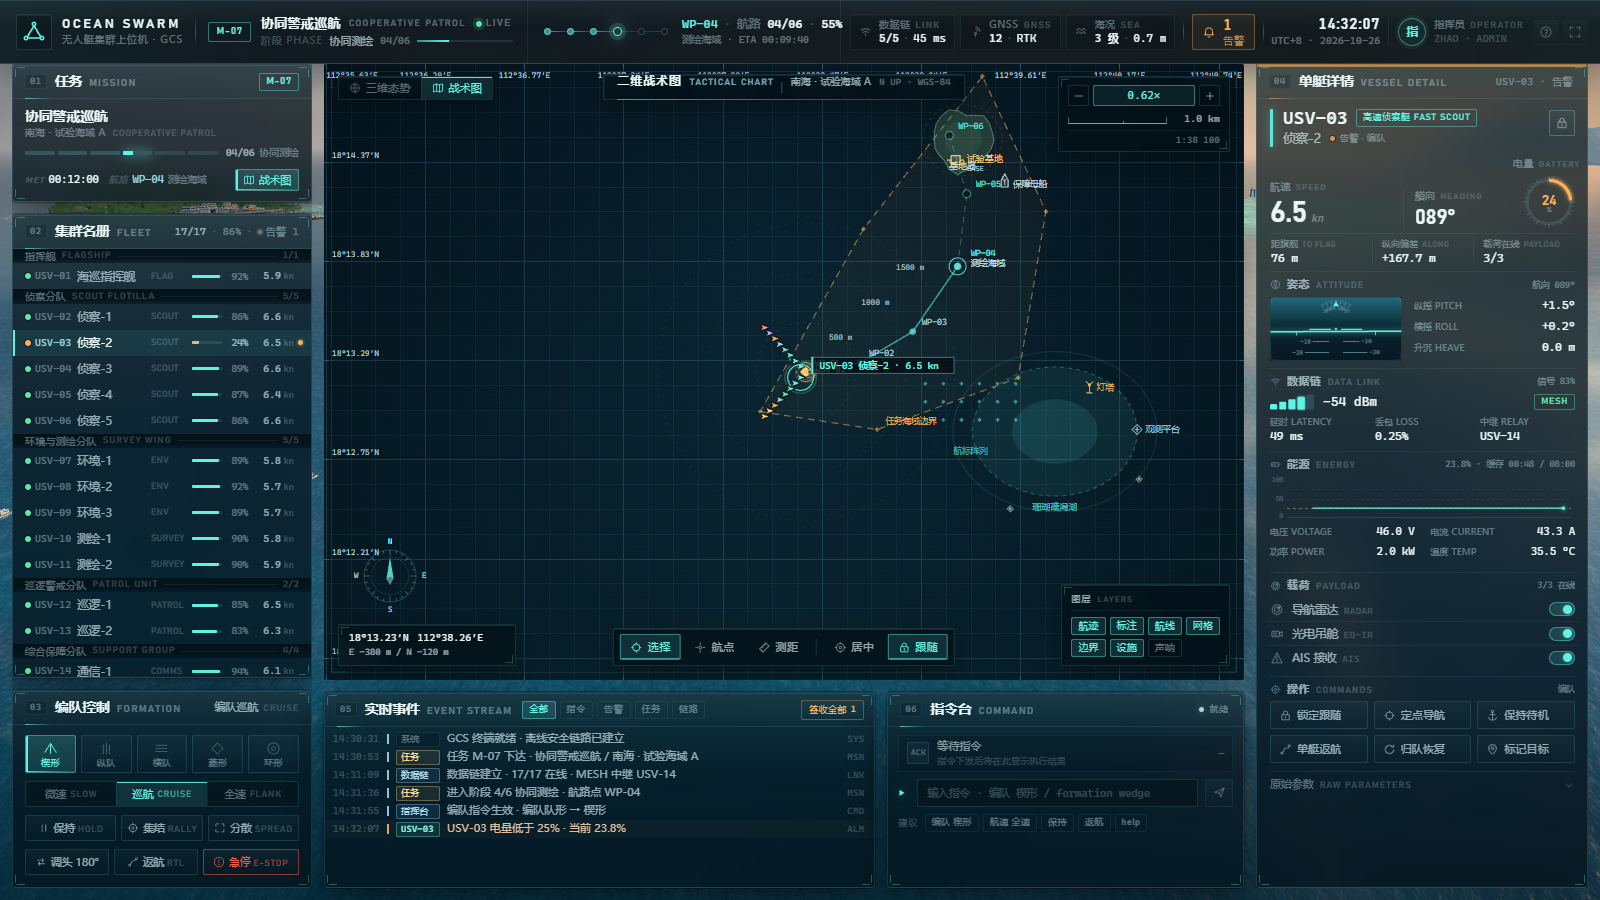
\includegraphics[width=\linewidth]{figures/gcs-02-map.png}
  \caption{二维战术图：海域边界、航路、17 艇位置与航迹、航点工具。}
  \label{fig:gcs-map}
\end{figure}

\subsection{交互与指令台}

三维拾取使用射线检测，选中后在船体上方显示带呼号与航速的锁定框。双击名册行或三维艇切换锁定跟随，按 \texttt{R} 返回编队跟随。中央 HUD 显示罗经带、当前视角、经纬坐标、航速与比例尺。

底栏指令台支持中英文命令。输入内容经过解析、校验与防抖后进入指令总线；在途阶段显示等待回执，成功后高亮对应面板并写入事件流，失败时显示拒绝原因。命令历史与建议 chips 帮助操作员快速执行常用指令。

\subsection{开机、急停与帮助}

首次进入时播放约 6~s 的开机自检动画，依次显示渲染器、场景、数据链、遥测与告警模块的自检状态，随后淡出。急停需要长按约 0.9~s 才生效，弹层内显示进度环、倒计时与松手取消提示。急停生效后顶栏出现红色告警，全部推进器停止，艇按阻力滑行并随流漂移；除解除急停外的指令都会被拒绝。帮助弹层列出鼠标、键盘与指令台的操作说明。

\begin{figure}[H]
  \centering
  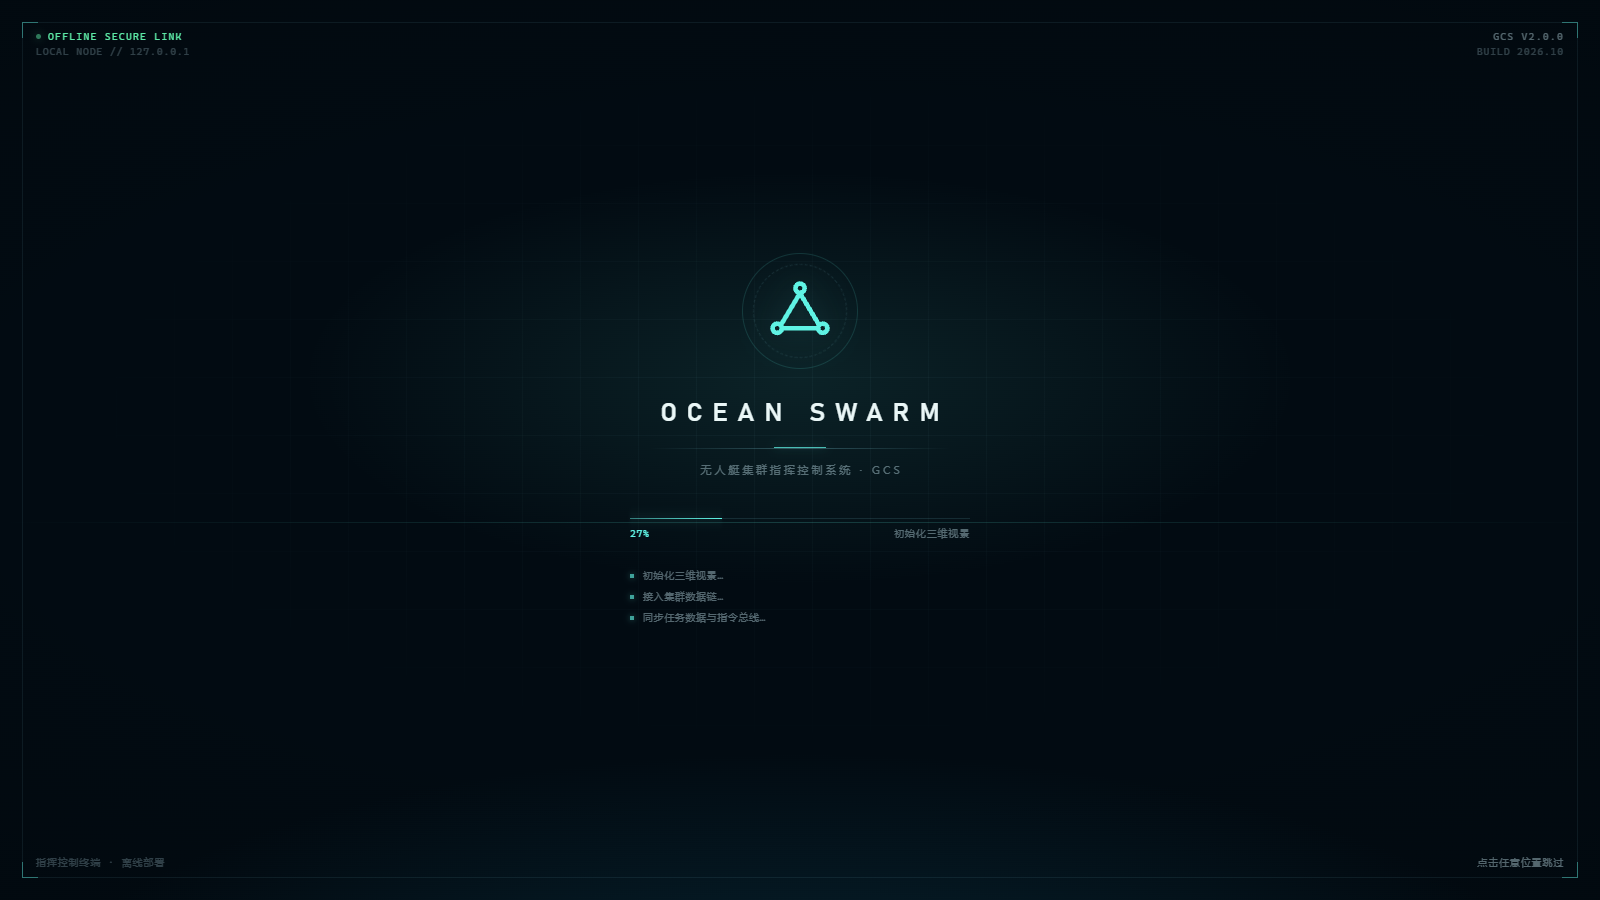
\includegraphics[width=0.92\linewidth]{figures/gcs-04-boot.png}
  \caption{开机自检界面。}
  \label{fig:boot}
\end{figure}

\begin{figure}[H]
  \centering
  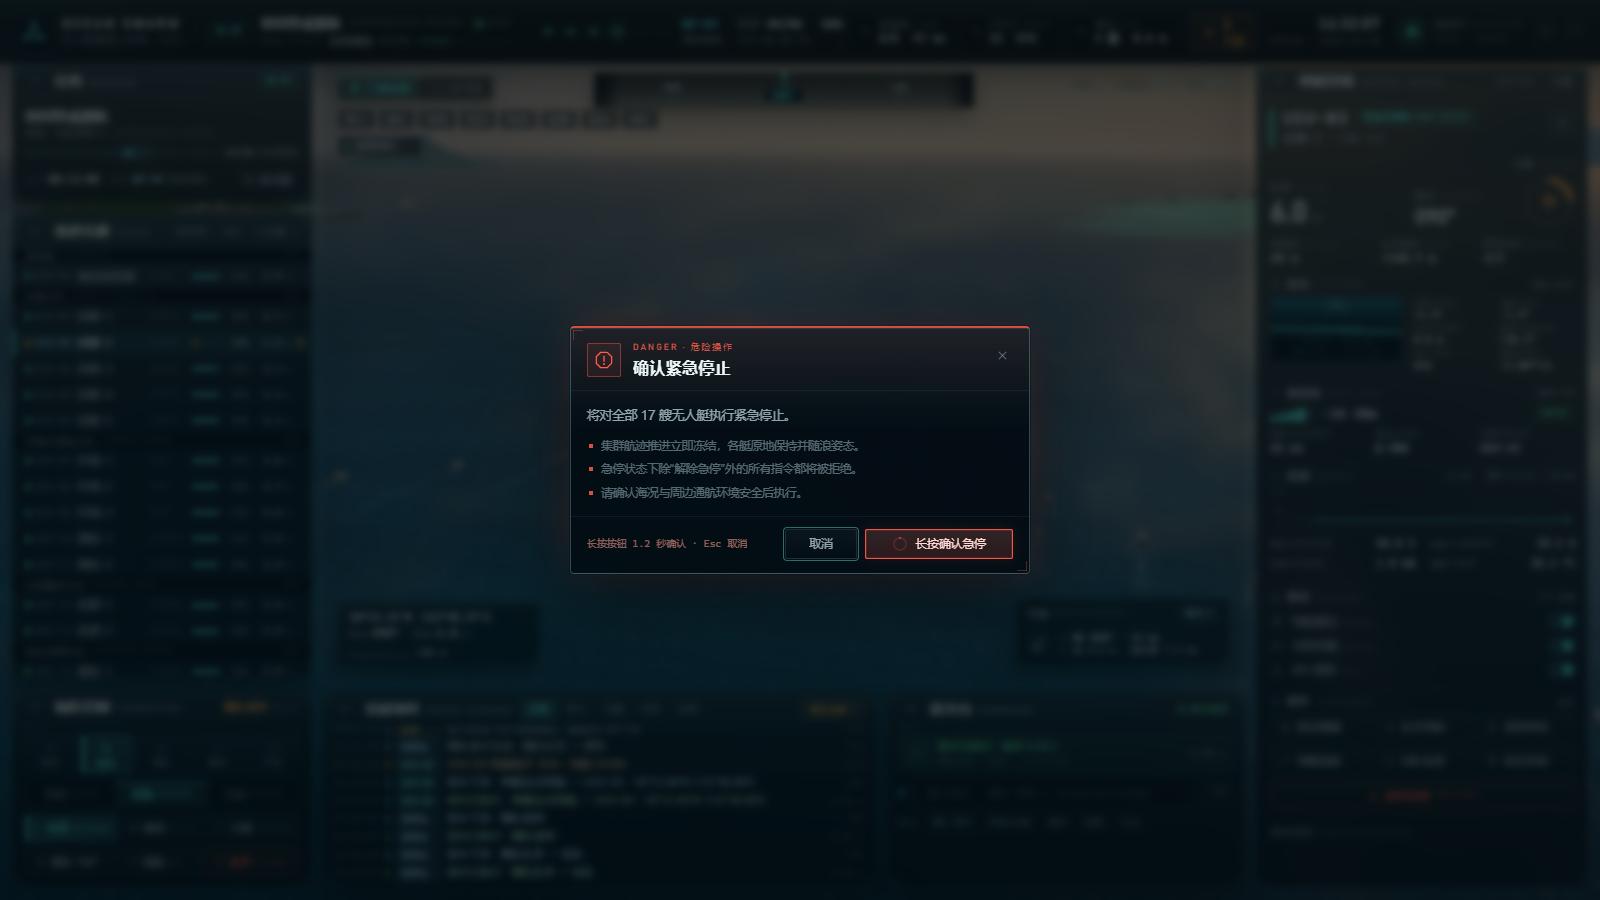
\includegraphics[width=0.9\linewidth]{figures/gcs-03-estop.png}
  \caption{急停长按确认覆盖层。}
  \label{fig:estop}
\end{figure}

纯净视景模式隐藏全部面板，保留三维场景与海鸥等环境动画，用于演示与截图。

% -----------------------------------------------------------------------------
\section{仿真与数据链}

\subsection{遥测模型}

仿真层以 10~Hz 生成快照。每艘艇维护位置、航向、航速、电量、温度、链路与载荷状态。舰速、航向、舵角、油门、漂角等字段直接读取场景真值；电量按任务负荷与时间缓慢下降，链路延时在 220 到 650~ms 之间波动，丢包与中继状态随机变化。任务阶段按航路点循环推进，MET 与 UTC+8 时间持续累计。

载入历史状态时，仿真层会先把电源与热模型收敛到巡航工作点，使首屏读数呈现稳定状态。

\subsection{指令生命周期}

\begin{table}[H]
\centering
\caption{指令从下发到执行完成的阶段}
\label{tab:cmd-lifecycle}
\small
\begin{tabular}{@{}p{0.18\linewidth}p{0.74\linewidth}@{}}
\toprule
\textbf{阶段} & \textbf{行为} \\
\midrule
校验 & 急停门禁、参数范围、目标存在性、重复防抖。非法指令立即返回拒绝原因。 \\
下发 & 生成带序号的在途命令，按数据链参数增加延时，可能产生丢包与重传。 \\
执行 & 编队控制层修改队形、航速或任务状态，单艇任务生成航点与到达判据。 \\
回执 & 成功或失败回执返回指令台与事件流，记录耗时与链路延时。 \\
反馈 & 场景运动与遥测更新，相关面板在下一帧或下一个快照中刷新。 \\
\bottomrule
\end{tabular}
\end{table}

指令类型包括队形切换、航速、编队保持与恢复、集结与分散、调头、返航、急停与解除、单艇派遣、单艇待机与载荷开关。每条指令都记录来源、时间、结果与动作描述，可在事件流中查询。

\subsection{告警}

告警引擎维护五类规则：低电量、链路异常、阵位偏离、艇离线、集群急停。低电量按阈值分级，电量继续下降时升级为严重告警；链路异常覆盖延时、丢包与离线；阵位偏离使用 30~m 警告与 70~m 严重阈值，条件需要持续 3~s 才成立；编队机动期间阵位告警挂起，避免换形过程产生误报。每条告警都有触发、升级、降级、恢复四类事件，恢复后从活动列表移除。

\subsection{确定性与复现}

仿真使用固定种子的随机数生成器。给定种子与相同操作序列，遥测、告警与事件流在同一模拟时刻保持一致。暂停功能冻结仿真时间，相机与界面保持响应；冻结功能同时停止渲染，供截图脚本在任意中间态取图。整机回归使用固定种子与冻结渲染，断言结果可重复。

% -----------------------------------------------------------------------------
\section{编队指挥控制}

\subsection{队形与阵位}

编队控制维护五种队形：楔形、纵队、横队、菱形、环形。旗舰位于阵位原点，16 艘护航艇按队形函数生成阵位坐标。阵位坐标位于编队路径坐标系，前向与右向分别为 $+$。队形支持 0.45 到 1.9 倍速巡航，队形尺度可在 0.2 到 3 倍之间调整。

\begin{figure}[H]
  \centering
  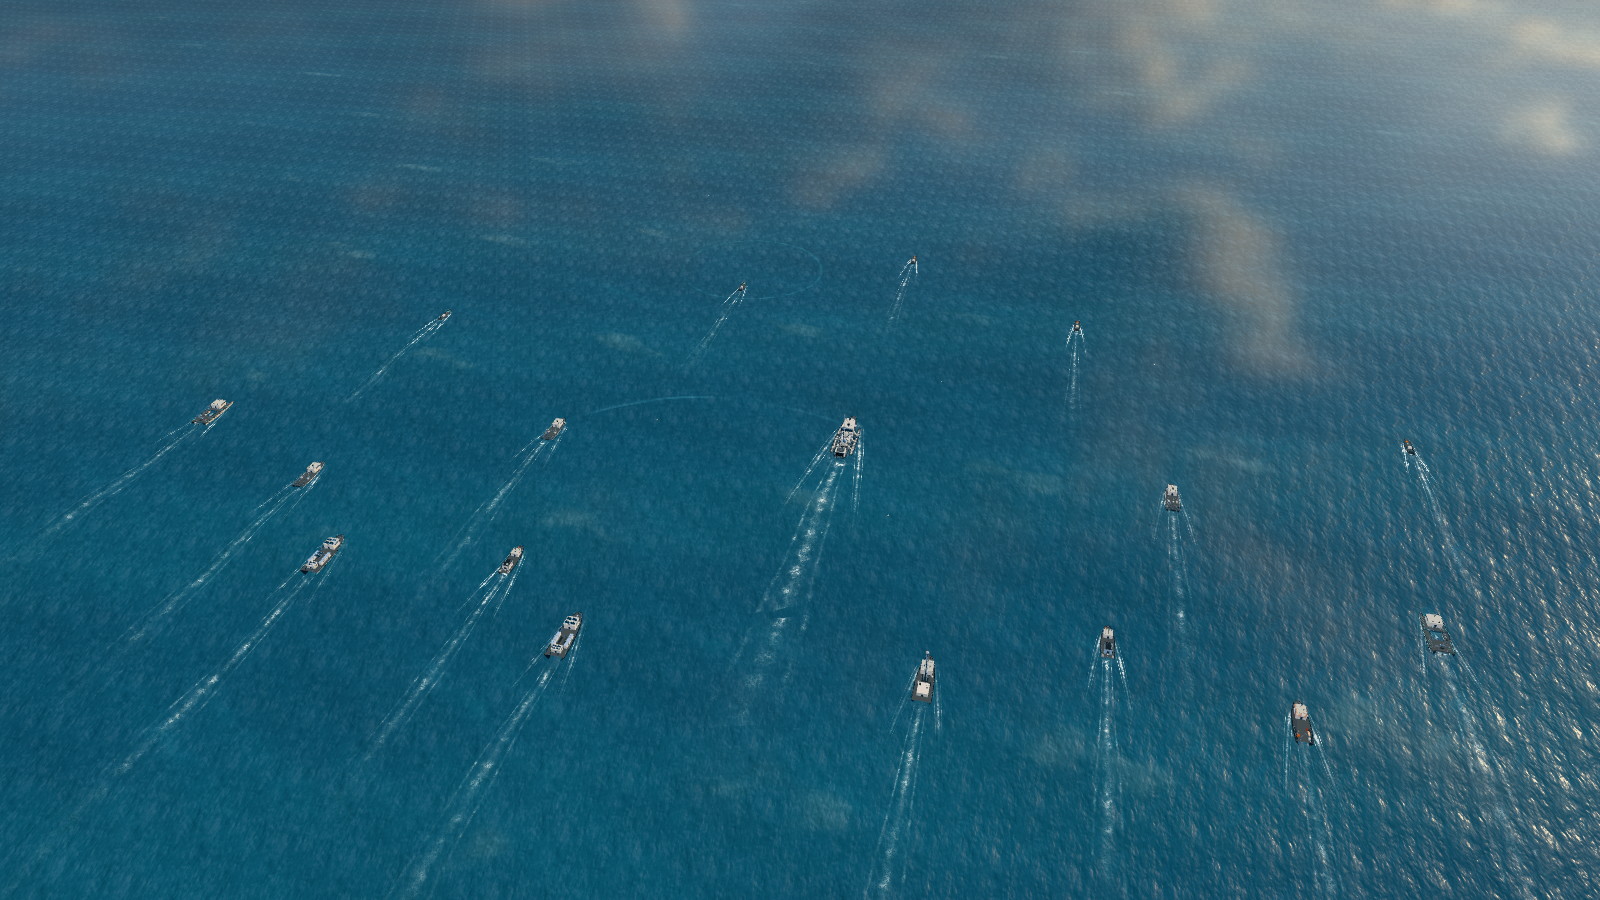
\includegraphics[width=0.95\linewidth]{figures/fig-02-fleet.png}
  \caption{高空俯视下的编队与尾迹。}
  \label{fig:fleet}
\end{figure}

\subsection{航速、保持与恢复}

航速指令调整编队巡航速度，速度变化由水动力模型逐步响应。保持指令冻结编队路径推进，各艇转入动力定位，围绕当前阵位保持位置与艏向；恢复指令解除冻结，编队继续沿航路前进。集结与分散通过调整队形尺度实现。

\subsection{调头与返航}

调头指令使编队按固定转向速率改变航向，累计转过约 180$^\circ$ 后回到巡航。返航指令把航路目标切换到试验基地，编队转向并保持航速前进，距离基地小于 140~m 时自动转入保持状态并提示到达。编队级转向速率限制在 0.03~rad/s 以内，返航纠偏限制在 ±0.015~rad/s，避免低速保障艇在急转中掉队。

\subsection{急停与恢复}

急停指令切断全部推进器与舵机，艇失去动力后按阻力滑行，随后随水流漂移。解除急停恢复编队与航速，各艇重新加速。急停期间除解除指令外的所有命令都被拒绝，拒绝原因写入指令台。

\subsection{单艇派遣}

单艇派遣把选中艇从编队中独立出来，按航点制导前往目标位置。制导使用制动包线，接近目标时减速；进入 18~m 范围后交给动力定位，艇在目标点附近保持。右栏状态显示自主模式与目标距离，到达后回到待机。

\begin{figure}[H]
  \centering
  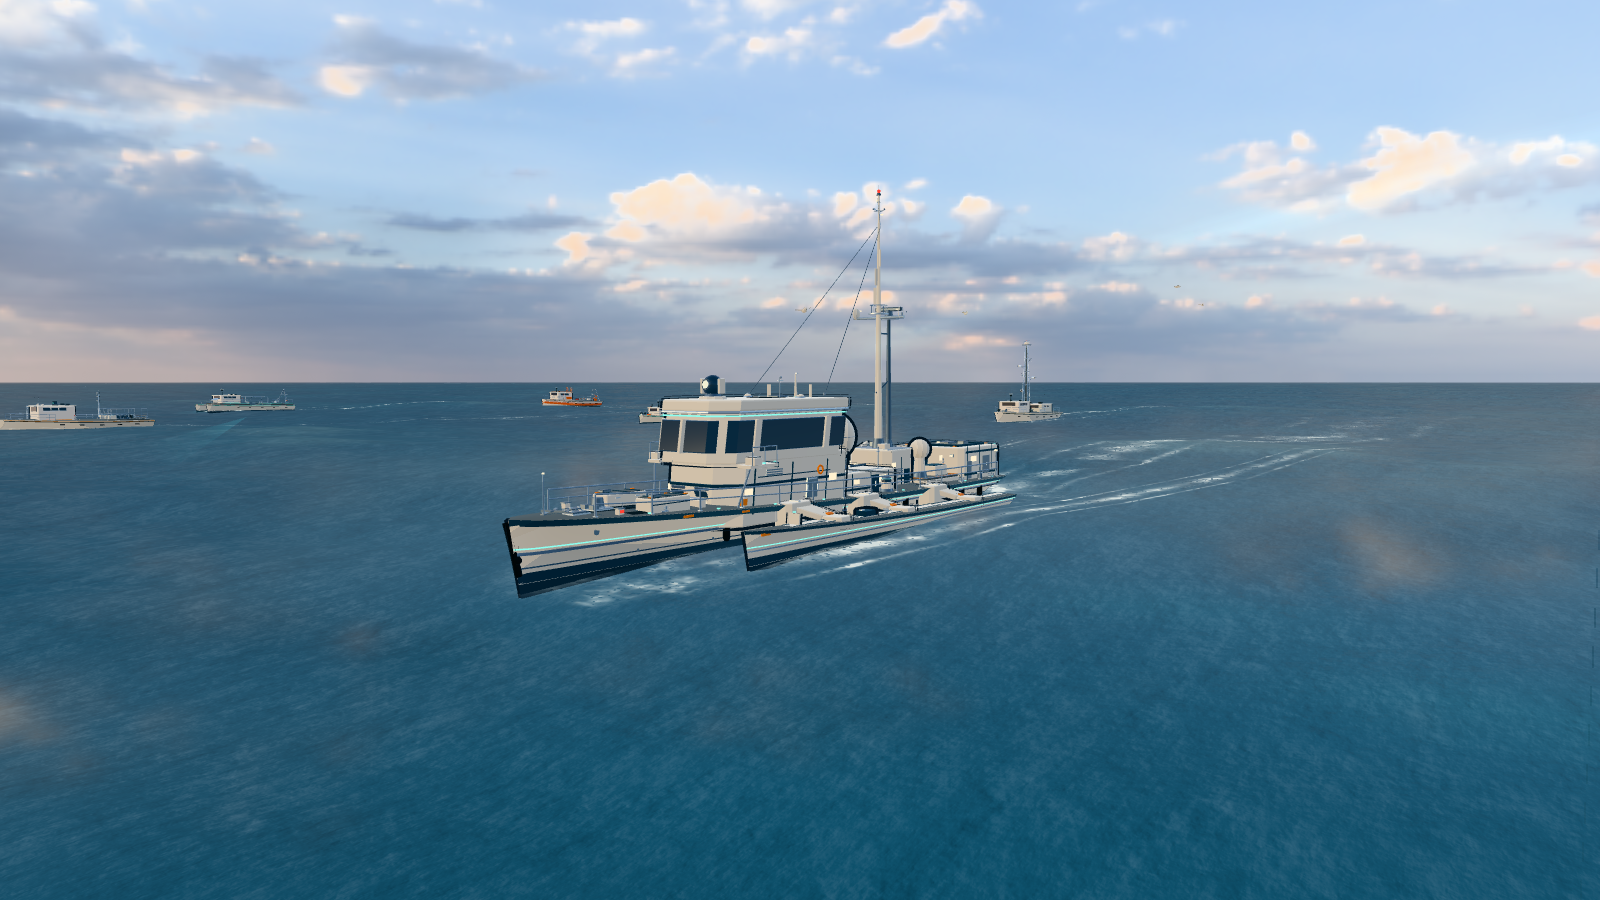
\includegraphics[width=0.95\linewidth]{figures/fig-06-bow.png}
  \caption{旗舰船首近景。}
  \label{fig:bow}
\end{figure}

\subsection{换形匹配与机动包线}

切换队形时，控制层按当前位置到新阵位的距离做全局匹配，把新阵位分配给最近的艇。楔形换纵队的场景中，若按名册顺序分配，部分保障艇会被排到几百米之后，只能等编队驶过再追赶；按最近匹配分配后，位移集中在阵位本身的变化上。即便采用最近匹配，单纵队对低速保障艇仍需要数分钟才能完成，这是水动力模型下的实际结果。

编队机动期间，控制层通过 \texttt{formationTransition} 与 \texttt{manoeuvring} 标志告知仿真层，阵位偏离告警在这段时间内挂起，换形结束后恢复判定。

% -----------------------------------------------------------------------------
\section{水动力动力学}

\subsection{状态与方程}

每艘艇的状态包含世界位置 $x,z$、艏向角 $\psi$、纵荡速度 $u$、横荡速度 $v$ 与艏摇角速度 $r$。体轴定义 $u$ 沿船首、$v$ 沿右舷、$r$ 以左转为正。

\begin{equation}
\dot x=\cos\psi\,u+\sin\psi\,v,\qquad
\dot z=-\sin\psi\,u+\cos\psi\,v,\qquad
\dot\psi=r .
\end{equation}

动力学采用刚体、附加质量与阻尼组合的形式，主机推力与舵力作为外部输入，$F_{dp}$ 与 $M_{dp}$ 为低速动力定位执行器的横向力与艏摇力矩：

\begin{equation}
\begin{aligned}
(m-X_{\dot u})\,\dot u &= (m-Y_{\dot v})\,v\,r + X_u\,u_r + X_{uu}\,u_r|u_r| + T,\\
(m-Y_{\dot v})\,\dot v &= -(m-X_{\dot u})\,u\,r + Y_v\,v_r + Y_{vv}\,v_r|v_r| + Y_\delta\sin\delta\,u_r^2 + F_{dp},\\
(I_z-N_{\dot r})\,\dot r &= (X_{\dot u}-Y_{\dot v})\,u\,v + N_r\,r + N_{rr}\,r|r| + N_\delta\sin\delta\,u_r^2 + M_{dp},
\end{aligned}
\label{eq:hydro}
\end{equation}

其中 $u_r=u-u_c(\psi)$、$v_r=v-v_c(\psi)$ 为相对水的速度，$\delta$ 为舵角，$T$ 为主机推力。积分在内部以不超过 0.02~s 的子步长执行，外层时间步 0.005 到 0.1~s 下保持稳定。

\subsection{执行器}

主机推力上限随艇型变化，范围 6.5 到 76~kN，油门经过一阶滞后，倒车推力为前进推力的固定比例。舵角限幅 $\pm30^\circ$，舵速率 25 到 40$^\circ$/s，舵伺服同样带一阶滞后。舵力与相对来流速度的平方成正比，低速时舵效下降，这一特性直接影响定点保持与低速机动。

低速动力定位执行器包含横向侧推与辅助艏摇两个通道。有效性随航速衰减：
\begin{equation}
e(u)=\mathrm{clamp}\!\left(1-\frac{|u|}{0.75\,U_{\max}},\,0.08,\,1\right).
\end{equation}
静止状态下，辅助艏摇通道可提供约 0.06 到 0.12~rad/s$^2$ 的角加速度；航速接近最大时，该通道的力矩不到满舵舵力矩的 5\%。

\subsection{水流}

试验海域设置 0.45~kn、210$^\circ$ 的水流。plant 的 $u,v$ 为对地速度，水流通过相对速度 $u_r,v_r$ 进入阻尼项，因此顶流航行时航迹向与艏向之间存在漂角，切断动力时艇随水流漂移。

\subsection{船型参数}

\begin{table}[H]
\centering
\caption{8 型无人艇参数}
\label{tab:usv-params}
\small
\begin{tabular}{@{}lrrrrrrr@{}}
\toprule
\textbf{型别} & 船长 (m) & 排水 (t) & 最大航速 (kn) & 推力 (kN) & 回转直径 & 巡航艏摇率 & 稳态漂角 \\
\midrule
旗舰 & 30.0 & 95 & 20 & 76 & 4.0 L & 2.95$^\circ$/s & 8$^\circ$ \\
侦察 & 10.5 & 3.5 & 24 & 8.1 & 4.6 L & 7.49$^\circ$/s & 13$^\circ$ \\
环境 & 16.5 & 9 & 16 & 7.6 & 4.1 L & 5.36$^\circ$/s & 9$^\circ$ \\
测绘 & 18.0 & 14 & 12 & 6.5 & 3.5 L & 5.61$^\circ$/s & 7$^\circ$ \\
巡逻 & 14.5 & 7.5 & 22 & 12.2 & 4.1 L & 6.10$^\circ$/s & 11$^\circ$ \\
通信 & 19.0 & 18 & 14 & 11.1 & 4.2 L & 4.43$^\circ$/s & 7$^\circ$ \\
能源 & 20.0 & 26 & 12 & 11.5 & 4.5 L & 3.93$^\circ$/s & 7$^\circ$ \\
救援 & 15.5 & 8 & 18 & 9.2 & 4.1 L & 5.71$^\circ$/s & 9$^\circ$ \\
\bottomrule
\end{tabular}
\end{table}

参数按真实量级设计：巡航速度 6~kn，最大航速 11 到 24~kn，全舵巡航回转直径 3.5 到 4.6 倍船长，稳态漂角 7 到 13$^\circ$，从静止加速到 80\% 最大航速需要 9.5 到 21~s。

\subsection{制导与自动舵}

编队制导在路径坐标系中计算前向与横向误差。横向误差通过前视点转换为期望艏向偏置，限幅 ±0.5~rad；前向误差转换为速度指令，同时设置速度下限，保证舵与侧推获得足够的来流。误差较大时启用侧推辅助，加快横向收敛。

速度环由前馈与比例积分组成。前馈通过 plant 的稳态反解得到油门，比例积分修正剩余误差，并限制超速追赶的幅度。艏向环输出期望艏摇率，舵角指令由期望角速度与角速度误差组合得到，最终受舵速率与机械限幅约束。

航点制导采用制动包线，期望速度随剩余距离减小，抵达 18~m 内交给动力定位。该流程使航点任务呈现减速、到达、稳定的完整过程。

\subsection{动力定位}

动力定位接收目标点与目标艏向，按以下步骤计算执行器指令：

\begin{enumerate}
  \item 位置误差乘以增益得到期望对地速度，进入 1.3~m 死区后速度归零；
  \item 期望对地速度减去水流得到对水速度，旋转到体轴得到期望纵荡与横荡速度；
  \item 纵荡通道使用油门前馈与比例积分，横荡通道使用侧推比例控制；
  \item 艏向通道使用舵与辅助艏摇力矩组合，保持目标艏向。
\end{enumerate}

在 0.45~kn 水流下对 8 型艇各做 120~s 定点保持测试，最大位置误差 0.25 到 0.90~m，测试结束时误差不超过 0.02~m，艏向误差为 0$^\circ$。

\subsection{典型机动}

\begin{figure}[H]
  \centering
  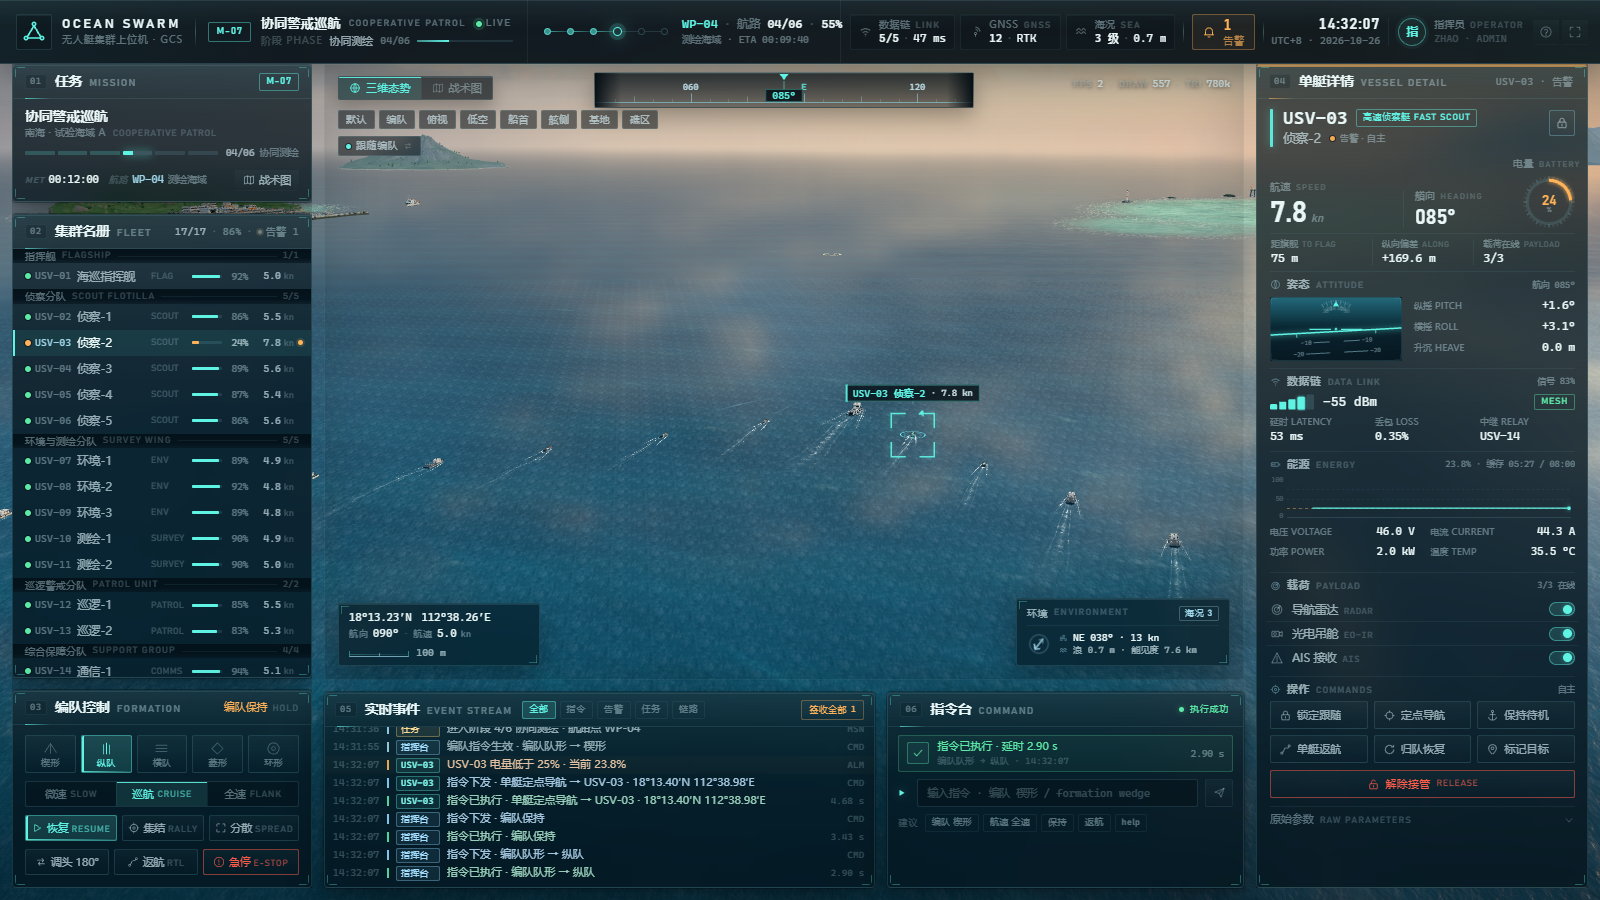
\includegraphics[width=\linewidth]{figures/gcs-05-formation.png}
  \caption{编队换形执行中的态势。右栏显示选中侦察艇的舵角、油门与艏摇率。}
  \label{fig:manoeuvre}
\end{figure}

\begin{table}[H]
\centering
\caption{水动力与运动闭环测试结果}
\label{tab:hydro-verify}
\small
\begin{tabular}{@{}p{0.30\linewidth}p{0.22\linewidth}p{0.40\linewidth}@{}}
\toprule
\textbf{测试} & \textbf{命令} & \textbf{结果} \\
\midrule
水动力模型 & \file{npm run qa:dynamics} & 141/141 通过：参数、加速、稳态、滑行、回转、漂角、水流、动力定位、数值稳定性 \\
闭环控制 & \file{npm run qa:motion} & 10/10 通过：巡航、航点到达、回转半径、动力切断漂移、17 艇编队收敛 \\
真实编队集成 & \file{npm run qa:fleet} & 13/13 通过：巡航 6.03~kn、阵位误差 13.4~m、漂角 4.2$^\circ$、航点到达 6.3~m、纵队收敛 17.9~m、调头误差 1.1$^\circ$、返航距离 2627 到 406~m \\
浏览器整机 & \file{npm run qa:gcs} & 30/30 通过：面板、遥测、交互、回执、急停、战术图，控制台零错误 \\
\bottomrule
\end{tabular}
\end{table}

\subsection{模型边界}

模型只覆盖水平面三个自由度，纵摇、横摇与升沉由波场采样驱动，未建立耐波性动力学。水动力系数按目标回转直径、漂角与加速时间反推，属于工程近似。波浪漂移力、风载荷、浅水效应与搁浅未纳入模型。编队变换使用轻量分离偏置，未实现严格避碰。这些边界在代码注释与本文中均有说明。

% -----------------------------------------------------------------------------
\section{性能与质量}

\subsection{优化措施}

\begin{itemize}
  \item 静态几何按材质合批，单艇约 20--25 次绘制调用；树木、珊瑚、海草、鱼群、浮标与风机叶片使用 InstancedMesh。
  \item 关闭实时阴影，使用尾迹泡沫、水线压暗与边缘光表达体积。
  \item 设备像素比上限 1.75，面板 Canvas 上限 2，控制填充率与内存占用。
  \item 遥测快照 10~Hz，面板只写变化的文本节点；战术图与仪表使用离屏 Canvas，避免逐帧重建 DOM。
  \item 七个面板按需动态加载，首屏不加载隐藏面板。
  \item 尾迹、海鸥、鱼群与选中光效使用预分配缓冲，循环内不创建对象。
  \item HDR 全景只解码一次，天空、海面与 PMREM 环境图共享同一张纹理，装配前完成预加载。
\end{itemize}

\subsection{实测数据}

测试环境为无头 Chromium 与 SwiftShader 软件渲染，窗口 1600$\times$900。软件渲染的帧率不代表真实 GPU 表现，绘制调用、三角形数量、资源加载与构建体积具有参考价值。

\begin{table}[H]
\centering
\caption{实测指标（v2.1）}
\label{tab:perf}
\small
\begin{tabular}{@{}l l p{0.36\linewidth}@{}}
\toprule
\textbf{指标} & \textbf{数值} & \textbf{说明} \\
\midrule
绘制调用 & 约 573 & 单帧提交，随视角变化 \\
三角形数量 & 约 80.5 万 & 单帧提交 \\
纹理 & 5 张 & HDR 全景、水面法线、梯度与噪声 \\
无人艇 & 17 艘 & 全部运行 3-DOF plant \\
控制台错误 & 0 & 页面异常、资源失败、着色器错误均为零 \\
外部网络请求 & 0 & 资源全部同源加载 \\
界面断言 & 30/30 & 面板、遥测、交互、回执、急停、战术图、纯视景 \\
软件渲染帧率 & 2--17~fps & 仅用于同条件对比 \\
生产构建 & 约 5.69~MB & JS 约 707~KB（gzip 207~KB）与本地素材 \\
\bottomrule
\end{tabular}
\end{table}

\subsection{自动化验证}

仓库提供六套验证脚本，全部位于 \file{artifacts/}，不参与生产构建：

\begin{enumerate}
  \item \file{npm run qa:gcs}：整机回归。Playwright 从冷启动加载页面，检查七个面板、DOM 数值、17 艇遥测与操纵量、名册与三维与右栏联动、战术图、航点派遣、编队回执、急停长按、帮助、纯视景、开机门闩、三维拾取、键盘快捷键与急停门禁，同时输出十张截图基线。
  \item \file{npm run qa:dynamics}：水动力自测，141 项断言。
  \item \file{npm run qa:motion}：plant 与 autopilot 闭环自测，10 项断言。
  \item \file{npm run qa:fleet}：使用 three.js 数学类在 Node 中驱动真实 Fleet 与 SwarmControl，13 项断言。
  \item \file{npm run qa:sim}：仿真引擎自测，32 项断言，覆盖快照结构、指令校验、告警生命周期、暂停回执与确定性。
  \item \file{node artifacts/sim/browser-check.mjs}：浏览器内仿真集成，16 项断言。
\end{enumerate}

截图基线与文档插图由 \file{artifacts/gcs/capture.mjs} 全量回归、\file{artifacts/gcs/bootshot.mjs} 开机截图与 \file{artifacts/gcs/states.mjs} 状态截图生成。

\subsection{已知限制}

\begin{enumerate}
  \item 任务阶段按航路点循环推进，MET 持续累计；跨午夜时日期文本会滚动。
  \item 水深为近似场，隐式阵位偏离依赖场景提供的误差值；编队机动期间告警挂起。
  \item 水动力模型为水平面三自由度，纵摇、横摇与升沉由波场驱动；系数为工程近似。
  \item 大幅换形与急停后的滑行时间较长，与真实小艇与保障艇的惯性有关。
  \item 软件渲染帧率较低时，数据链回执的墙钟观测可能顺延到下一界面帧，仿真时间语义保持一致。
  \item 默认观察距离下 10 到 30~m 的艇在屏幕中较小，可通过视角预设或滚轮拉近观察。
  \item 战术图在 2.2 倍以上缩放时，编队内的 17 个呼号标签会变得拥挤。
  \item 项目为离线仿真演示，数据链、告警与任务阶段由确定性模型生成，未连接真实艇端。
\end{enumerate}

% -----------------------------------------------------------------------------
\section{项目交付}

v2.1 交付一套可运行的无人艇集群上位机、完整的三维海域视景、仿真数据链、编队控制与水动力动力学，以及配套的验证脚本与文档。主要文件与目录见附录 C。

后续工作可以从三个方向展开：接入真实艇端遥测与指令协议，把水动力模型扩展到六自由度并加入耐波性，以及在编队控制层加入更严格的多艇避碰与任务规划。

\vspace{0.8em}
\noindent 仓库地址：\repolink

\noindent 架构细节见 \file{docs/GCS-architecture.md}，设计系统见 \file{docs/GCS-design-system.md}。

% ============================= 附录 =========================================
\appendix

\section{波场采样与随浪姿态}

船体随浪姿态由波场采样得到。取船首、船尾、左舷、右舷四个点与船中点的水面高度，按船长与型宽计算纵摇与横摇：
\begin{equation}
\begin{aligned}
\text{pitch}^{\ast} &= \arctan\frac{h_{bow}-h_{stern}}{2L_h}\,\gamma_p + \text{planing},\\
\text{roll}^{\ast} &= -\arctan\frac{h_{right}-h_{left}}{2B_h}\,\gamma_r + \text{bank},\\
h_{heave}^{\ast} &= 0.35\,h_c + 0.1625\,(h_b+h_s+h_r+h_l),
\end{aligned}
\label{eq:attitude}
\end{equation}
其中 $\gamma_p,\gamma_r$ 为按艇型配置的响应系数，快速艇接近 1，双体测绘艇约 0.4。升沉、纵摇与横摇经过指数平滑，避免数值抖动。该计算与水平面运动相互独立。

\section{素材与许可}

\begin{itemize}
  \item 天空 HDR 全景：Poly Haven “Kloppenheim 06 (Pure Sky)”，CC0 1.0，2048$\times$1024 RGBE，随仓库分发。
  \item 水面法线贴图：three.js 官方示例素材，MIT 许可，1024$\times$1024，随仓库分发。
  \item 三维场景代码与上位机代码：本项目仓库，详见 \file{CREDITS.md}。
\end{itemize}

\section{目录结构}

\begin{lstlisting}[language=bash, caption={仓库目录结构（节选）}]
ocean-swarm-gcs/
  index.html
  package.json / vite.config.js / README.md / CREDITS.md
  docs/
    OceanSwarm-GCS-dev-doc.tex   # 本文档
    OceanSwarm-GCS-dev-doc.pdf
    GCS-architecture.md / GCS-design-system.md
    figures/                     # 场景图与 GCS 截图基线
  public/hdr/                    # 本地 HDR 天空全景
  public/textures/               # 本地水面法线贴图
  src/main.js                    # 场景装配、GCS 集成、镜头、拾取
  src/config.js                  # 调色板、布局、名册、水流、光照
  src/core/                      # 几何、HDR、材质、波场、海面、天空
  src/objects/                   # ships / world / effects
  src/systems/
    formation.js                 # 航线、阵位与随浪姿态
    vessel-dynamics.js           # 3-DOF 水动力 plant
    motion-controller.js         # 制导、速度环、艏向环、动力定位
    swarm-control.js             # 编队、航速、保持、调头、返航、急停、单艇任务
    camera-director.js           # 镜头导演
  src/gcs/                       # 领域常量与场景真值适配
  src/sim/                       # 遥测、数据链、告警、事件与时钟
  src/ui/                        # 界面根、七个面板、Canvas 仪表与样式
  artifacts/                     # QA 脚本与截图产物（不参与构建）
\end{lstlisting}

\vfill
\begin{center}
{\small\color{themegray}
文档结束 · 2026 年 10 月 26 日 · 朱华天\\[0.3em]
\repolink}
\end{center}

\end{document}

